\documentclass{beamer}
%\usetheme{Berlin}
%\usetheme{Ilmenau}
%\usetheme{Dresden}
%\usetheme{Berkeley}
%\usetheme{Bergen}
%\usetheme{Boadilla}
%\usetheme{Copenhagen}
%\usetheme{Hannover}
%\usetheme{Luebeck}
%\usetheme{AnnArbor}
%\usetheme{Darmstadt}
%\usetheme{Frankfurt}
\usetheme{Madrid}%azulito-li;la
%\usetheme{Warsaw}%int
%\usetheme{Antibes}
%\usetheme{CambridgeUS}%rojo-gris
%\usetheme{Malmoe}
%\usetheme{PaloAlto}

\usepackage{graphicx}
\usepackage{adjustbox}
\usepackage[utf8]{inputenc}
\usepackage[spanish]{babel}
\usepackage{url}
\usepackage{multirow}
\usepackage{booktabs}
%\usepackage{beamerthemeshadow}
\usepackage{caption}


\hyphenation{}


%Arreglos en el footnote
\makeatletter
\setbeamertemplate{footline}
{
  \leavevmode%
  \hbox{%
  \begin{beamercolorbox}[wd=.333333\paperwidth,ht=2.25ex,dp=1ex,center]{author in head/foot}%
    \usebeamerfont{author in head/foot}\insertshortauthor
  \end{beamercolorbox}%
  \begin{beamercolorbox}[wd=.58\paperwidth,ht=2.25ex,dp=1ex,center]{title in head/foot}%
    \usebeamerfont{title in head/foot}\inserttitle
  \end{beamercolorbox}%
  \begin{beamercolorbox}[wd=.1\paperwidth,ht=2.25ex,dp=1ex,center]{date in head/foot}%
    \usebeamerfont{date in head/foot}\insertframenumber{} / \inserttotalframenumber\hspace*{2ex} 
  \end{beamercolorbox}}%
  \vskip0pt%
}
\makeatother

%Apagar el menu de presentacion
\setbeamertemplate{navigation symbols}{}

\begin{document}
\title{Optimización de viajes compartidos en taxis utilizando algoritmos evolutivos}
\author[G. Fagúndez \and R. Massobrio]{Gabriel Fagúndez de los Reyes \and Renzo Massobrio} 
\institute[]{Facultad de Ingeniería,\\
Universidad de la República,\\
Montevideo, Uruguay}

\pgfdeclareimage[height=1.7cm]{university-logo}{logo}
\titlegraphic{\pgfuseimage{university-logo}}
\date{}

\frame{\frametitle{}\titlepage} 
\frame{\frametitle{Contenido}\tableofcontents} 

% Pausas transparentes
\setbeamercovered{transparent}




% Slide - Introducción ==============================================================
\section{Introducción}
\frame{\tableofcontents[currentsection]}

\frame{
	\frametitle{Motivación} 
	\begin{block}{Car pooling}
		\begin{itemize}
			\item Beneficios en el plano ecológico y económico, individuales y colectivos.
			\item Iniciativas para atender el interés del público: carriles exclusivos, campañas para compartir los viajes al trabajo y aplicaciones para encontrar compañeros de viaje.
		\end{itemize}
	\end{block}
	
	\pause 
	
	\begin{block}{Taxi pooling}
		\begin{itemize}
			\item Los taxis son un medio de transporte rápido y confiable, especialmente en ciudades donde el transporte público es poco eficiente.
			\item Los taxis raramente viajan a capacidad completa, impactando en la congestión del tráfico y en la contaminación de las ciudades.
			\item Tarifas altas desalientan a los usuarios.
			\item \alert{15\%} de los accidentes fatales en Uruguay involucran a un conductor alcoholizado (UNASEV).
		\end{itemize}
	\end{block}
}




% Slide - Definición del problema ==============================================================
\section{Definición del problema} 
\frame{\tableofcontents[currentsection]}

\frame{
	\frametitle{Descripción del problema}
	\begin{block}{Problema de viajes compartidos en taxis (PVCT)}
		Un grupo de personas ubicadas en un \textbf{mismo lugar de origen}, desean viajar hacia \textbf{diferentes destinos} utilizando taxis de forma compartida.

		Se busca determinar la cantidad de taxis, la asignación de pasajeros y las rutas a seguir, de forma de \alert{minimizar el costo total del grupo de pasajeros}.
	\end{block}
	
	\pause
	
	\begin{block}{Consideraciones}
		\begin{itemize}
			\item Cada taxi puede trasladar a un número limitado de pasajeros.\pause
			\item El número máximo de taxis para $N$ pasajeros es $N$.\pause
			\item Costo de un taxi = \textbf{costo inicial} (“bajada de bandera”) $+$ \textbf{costo determinado por la distancia}. \pause
			\item No se consideran otros posibles costos (e.g. esperas, propinas, peajes).
		\end{itemize}		
	\end{block}
}

\frame{
	\frametitle{Formulación del problema}
	\begin{itemize}
		\item Un conjunto de pasajeros $P = \{p_1,p_2,\ldots,p_N\}$ que viajan desde un origen común $O$ a un conjunto de destinos $D = \{d_1,d_2,\ldots,d_N\}$.\pause

		\item Un conjunto de taxis $T = \{t_1,t_2,\ldots,t_M\}$; con $M \leq N$; y una función $C:T\rightarrow\{0,1,\ldots,C_{MAX}\}$ que indica la cantidad de pasajeros en un taxi. $C_{MAX}$ es la capacidad máxima permitida en un mismo taxi.\pause

		\item Una constante $B$ indica el costo inicial del taxi (``bajada de bandera'')\pause
		
		\item Una función de distancia, $dist: \lbrace \lbrace O \rbrace \cup D \rbrace \times D \rightarrow \mathbb{R}^+_0$.\pause
		
		\item Una función de costo asociado a la distancia recorrida por cada taxi, $cost: \mathbb{R}^+_0 \rightarrow \mathbb{R}^+_0$.
	\end{itemize}\pause

	Se desea hallar la planificación $f:P \rightarrow T \times \lbrace 1, \ldots,C_{MAX} \rbrace$
	que \alert{minimice la función de costo total ($CT$)}.
	\begin{equation*}
			CT  =  \sum\limits_{t_{i}, C(t_{i})\neq0} \Bigg[B+\sum\limits_{j=1}^{C(t_{i})}cost\bigg(dist \underbrace{\Big(dest\big(f^{-1}(t_{i},j-1)\big),dest\big(f^{-1}(t_{i},j)\big)\Big)}_{\text{destinos consecutivos en el recorrido del taxi } t_i}\bigg)\Bigg]
	\end{equation*}
}

% \frame{
% 	\frametitle{Variante multiobjetivo del PVCT}
% 	\begin{block}{Motivación}
% 		La decisión de un usuario puede estar condicionada a la demora que debe experimentar por compartir su viaje. 
% 		%Por tal motivo, es de interés estudiar 
% 		La variante multiobjetivo del problema minimiza simultáneamente el \alert{costo del grupo} de usuarios y la \alert{demora percibida} por cada uno de ellos.
% 	\end{block}
	
% 	\pause
	
% 	\begin{block}{Descripción}
% 		Se agrega un \textbf{``nivel de apuro''} asociado a cada pasajero, que denota la demora que está dispuesto a tolerar un usuario por compartir su viaje.
	
% 		Se contemplan \textbf{vehículos de distintas capacidades}, aportando mayor realismo a la formulación.
% 	\end{block}
% }

\frame{
	\frametitle{Variante multiobjetivo del PVCT: formulación matemática}
	Se busca minimizar simultáneamente el \alert{costo total} y la \alert{demora total}.\pause
	\begin{equation*}
			CT  =  \sum\limits_{t_{i}, C(t_{i})\neq0} \Bigg[B+\sum\limits_{j=1}^{C(t_{i})}cost\bigg(dist\overbrace{\Big(dest\big(f^{-1}(t_{i},j-1)\big),dest\big(f^{-1}(t_{i},j)\big)\Big)}^{\text{destinos consecutivos en el recorrido del taxi } t_i}\bigg)\Bigg]
	\end{equation*}\pause
	\begin{equation*}
		\begin{split}
			DT = \sum\limits_{t_{i}} \Bigg[\sum\limits_{j=1}^{C(t_{i})}\bigg[ &  \overbrace{\sum\limits_{h=1}^{j} time\Big(dest\big(f^{-1}(t_{i},h-1)\big), dest\big(f^{-1}(t_{i},h)\big)\Big)}^{\text{tiempo efectivo de traslado del pasajero en la posición } j \text{ del taxi } t_i} \\
			& - \underbrace{tol\big(f^{-1}(t_{i},j)\big) + time\Big(O, dest\big(f^{-1}(t_{i},j))\Big)}_{\text{tiempo tolerado por el pasajero en la posición } j \text{ del taxi } t_i}\bigg]\Bigg]
		\end{split}	
	\end{equation*}

	\begin{itemize}
		\item $time: \lbrace \lbrace O \rbrace \cup D \rbrace \times D \rightarrow \mathbb{R}^+_0$ indica el tiempo de recorrido.	
		\item $tol: P \rightarrow \mathbb{R}^+_0$  indica el tiempo adicional tolerado por cada pasajero.
	\end{itemize}
}

\frame{
	\frametitle{Complejidad del PVCT}
	\begin{block}{Complejidad}
	%El PVCT tiene varios puntos en común con dos conocidos problemas: el \textit{Car Pooling Problem (CPP)} y el \textit{Vehicle Routing Problem (VRP)}.

	Baldacci et al. (2004) estudiaron una variante del \textit{Car Pooling Problem (CPP)} donde trabajadores desean compartir vehículos hacia y desde el lugar de trabajo. 
	
	Esta variante es un caso particular del \textit{Vehicle Routing Problem (VRP)} con demanda unitaria, el cual es $\mathcal{NP}$--difícil [Letcheford et al. (2002)].
	\end{block}

	\pause

	\begin{block}{Estrategias de resolución}
	Cuando se utilizan instancias de tamaños realistas, los algoritmos exactos tradicionales no resultan útiles para una planificación eficiente.

	\alert{Heurísticas} y \alert{metaheurísticas} permiten calcular soluciones de calidad aceptable en tiempos razonables.
	\end{block}

}



% Slide - Trabajo relacionado ==============================================================
\section{Trabajo relacionado} 
\frame{\tableofcontents[currentsection]}

\frame{
	\frametitle{Trabajo relacionado}

	\begin{block}{Car pooling problem (CPP)}
	Yan et al. (2011) \textbf{CPP con histórico de viajes} (relajación lagrangeana). %Converge a menos de 3\% del óptimo en $\sim$1 hora (600 a 1400 pasajeros). 
	\end{block}
	\pause
	\begin{block}{Dial--a--ride problem (DARP)}
	Cordeau et al. (2003) \textbf{DARP estático con ventanas de tiempo}. \\\hspace{.8cm} {\small Búsqueda tabú con tiempos de ejecución de hasta 90 minutos.}
	\end{block}


	\pause
	\begin{block}{Taxi pooling problem (TPP)}
	Tao et al. (2007) Heurísticas ávidas para \textbf{one--to--many} y many--to--one. \\ \hspace{.8cm}{\small Las mejoras se reportan en términos absolutos.}

	Ma et al. (2013) TPP dinámico con pedidos en tiempo real.\\ \hspace{.8cm}{\small 13\% de ahorro en distancia con un algoritmo ávido en \textbf{instancias realistas}.}
	\end{block}

	\pause
	\begin{block}{Resumen}
	Pocos trabajos \alert{centrados en el usuario} y con un enfoque \alert{multiobjetivo}.
	\end{block}
}





% Slide - Implementación ==============================================================
\section{Implementación} 
\frame{\tableofcontents[currentsection]}

\frame{
	\frametitle{Algoritmos evolutivos}
	\begin{block}{Definición}
		\begin{itemize}
			\item Los \textit{algoritmos evolutivos} (AE) son técnicas estocásticas que emulan el proceso de evolución natural de las especies para resolver problemas de optimización, búsqueda y aprendizaje.\pause
			\item Un AE es una técnica iterativa (cada iteración se denomina \textbf{generación}) que aplica operadores estocásticos sobre un conjunto de individuos (la \textbf{población}).\pause
			\item Cada individuo en la población codifica una solución tentativa al problema y tiene un valor de \textbf{fitness}, dado por una función de evaluación que determina su adecuación para resolver el problema. \pause
			\item El propósito del AE es mejorar el fitness de los individuos en la población mediante la aplicación iterativa de \textbf{operadores evolutivos} a individuos seleccionados según su fitness, guiando al AE hacia soluciones tentativas de mayor calidad.
		\end{itemize}
	\end{block}
}


\frame{
	\frametitle{AE para el PVCT monoobjetivo}
	\begin{columns}[totalwidth=\linewidth]
	\column{0.43\linewidth}
		\begin{block}{Aspectos comunes}
		\begin{itemize}
		\item Tuplas de largo $2N-1$\\
		\hspace{.5cm}{\small$N=$ \#pasajeros.}
		\pause
		
		\item Inicialización:\\
		\hspace{.5cm}{\small aleatoria y ávida.}
		\pause
		
		\item Cruzamiento basado en posición (PBX).% + función correctiva.

		\pause
		\item Mutación por intercambio (EM).% + función correctiva.
		\pause


		\item Función correctiva:\\ \hspace{.5cm}{\small desplaza ceros para}\\ \hspace{.5cm}{\small romper secuencias de}\\ \hspace{.5cm}{\small dígitos inválidas.}
		\pause

		\item Implementados en Malva.
		\end{itemize}
		\end{block}

	\column{0.57\linewidth}
		\centering

		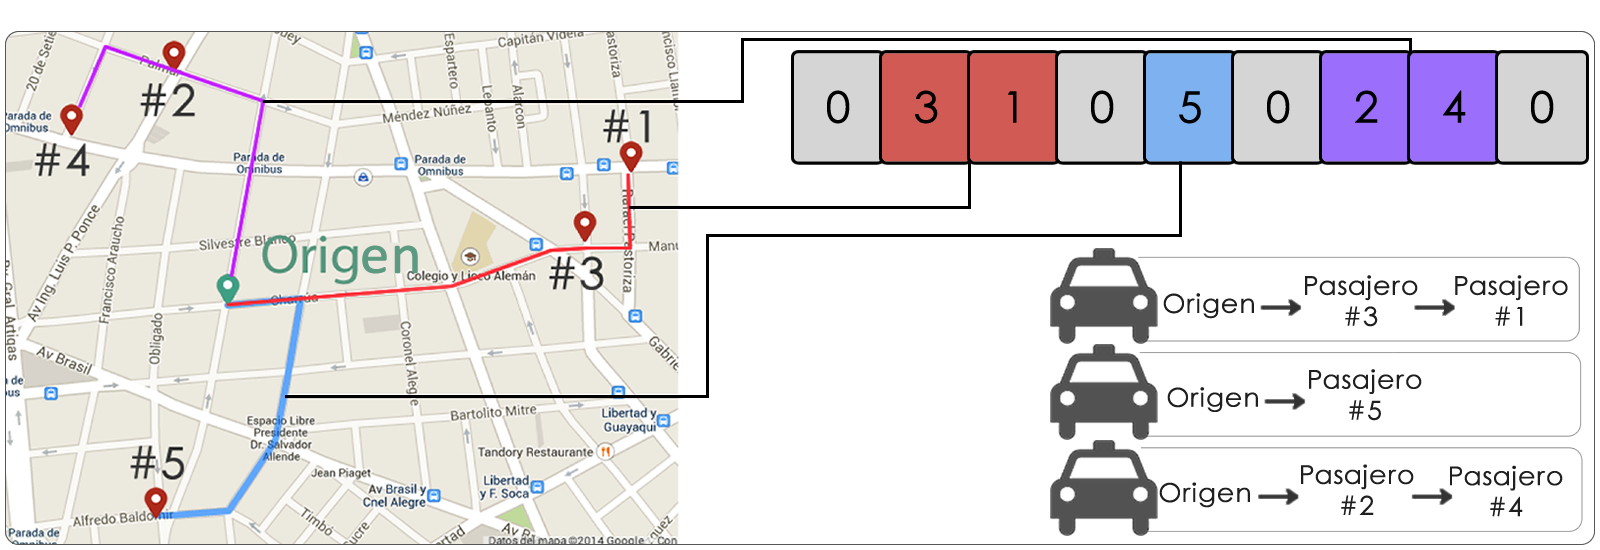
\includegraphics[width=0.9\textwidth]{distribucion.png}

		\only<1-2>{\mbox{\phantom{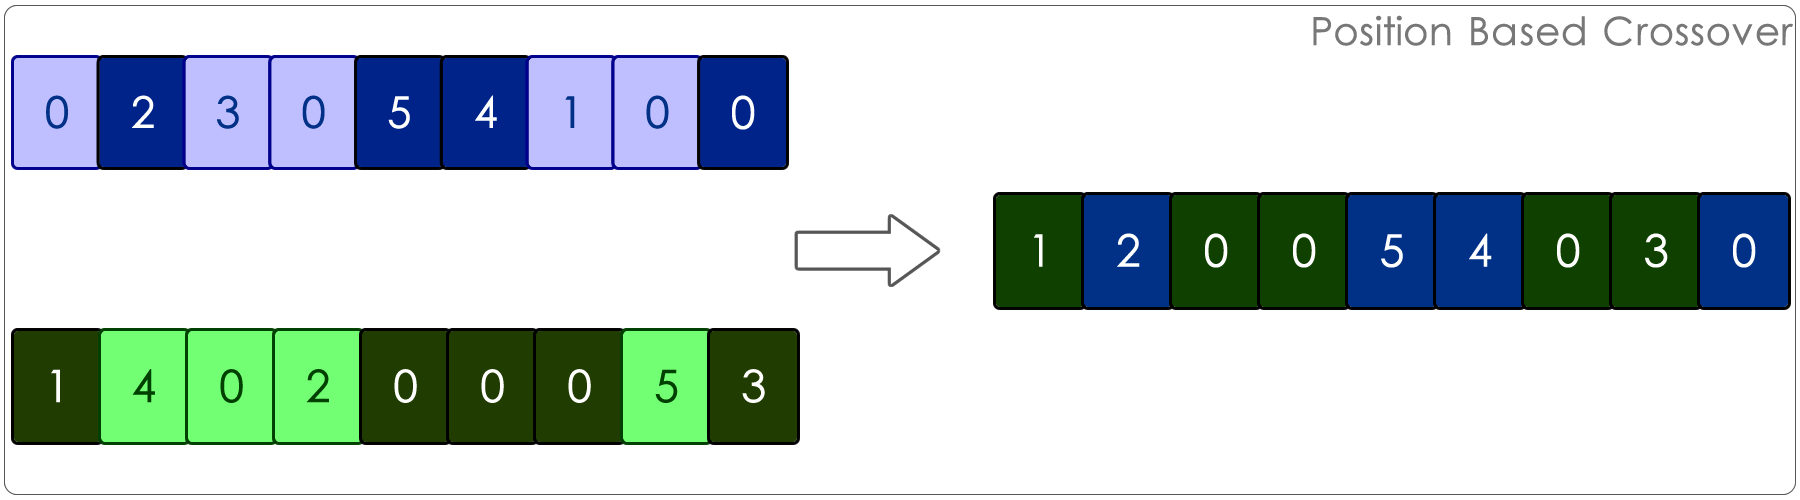
\includegraphics[width=0.9\textwidth]{pbx_simple.png}}}}
		\includegraphics<3->[width=0.9\textwidth]{pbx_simple.png}

		\only<1-3>{\mbox{\phantom{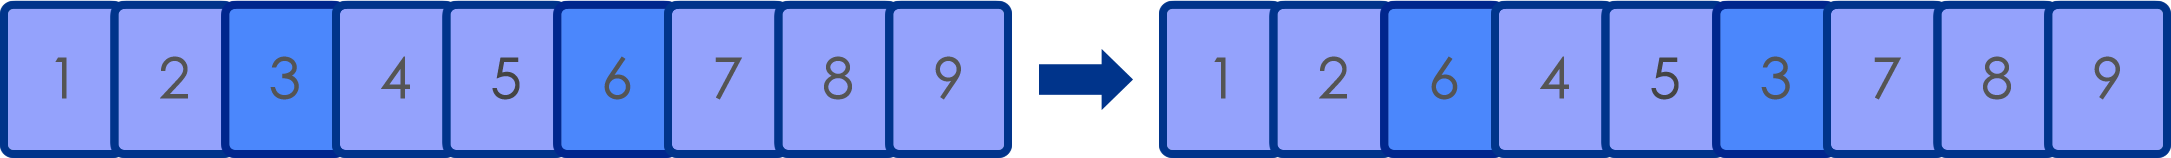
\includegraphics[width=0.9\textwidth]{em.png}}}}%
		\includegraphics<4->[width=0.9\textwidth]{em.png}

		\only<1-4>{\mbox{\phantom{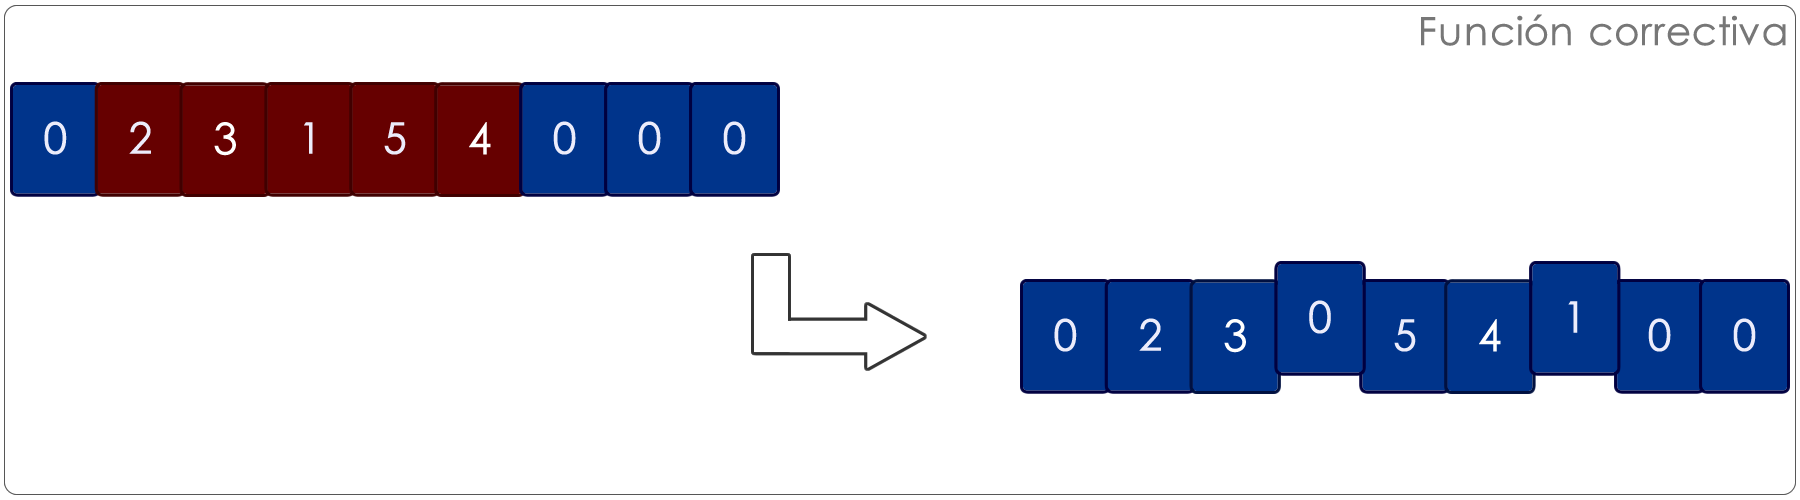
\includegraphics[width=0.9\textwidth]{temporal.png}}}}%
		\includegraphics<5->[width=0.9\textwidth]{temporal.png}
	\end{columns}

}

\frame{
	\frametitle{AE para el PVCT monoobjetivo}
	\begin{block}{\textit{seqEA}}
	AE \textbf{secuencial}. Utiliza selección proporcional.
	\end{block}
	\pause
	\begin{block}{Modelos paralelos en AE}
		Buscan \textbf{mejorar el desempe\~no} de los AE.\\
		\alert{Modelo de subpoblaciones distribuidas}: divide la poblaci\'on en \textbf{islas} % que ejecutan un AE secuencial e 
		que intercambian individuos mediante \textbf{migración}.
	\end{block}
	\pause
	\begin{columns}[totalwidth=\textwidth]
	\column{0.6\textwidth}
			\begin{block}{AE paralelo con micro--población (\textit{p$\mu$EA})}
				%Los AE con subpoblaciones distribuidas suelen perder diversidad. %, convergiendo a soluciones sub-óptimas del problema.
				\begin{itemize}
				\item Poblaciones pequeñas.% e incluye un \textbf{operador específico de diversidad}.% para mitigar este problema.
				\item Selección por torneo $(m,k)$.
				\item Migración asíncrona.
				\item Topología de anillo unidireccional.
				%\item Individuos a migrar seleccionados por torneo (reemplazan a los peores de la isla vecina).
				\end{itemize}
			\end{block}
	\column{0.4\textwidth}
		\centering
		\only<1,2>{\mbox{\phantom{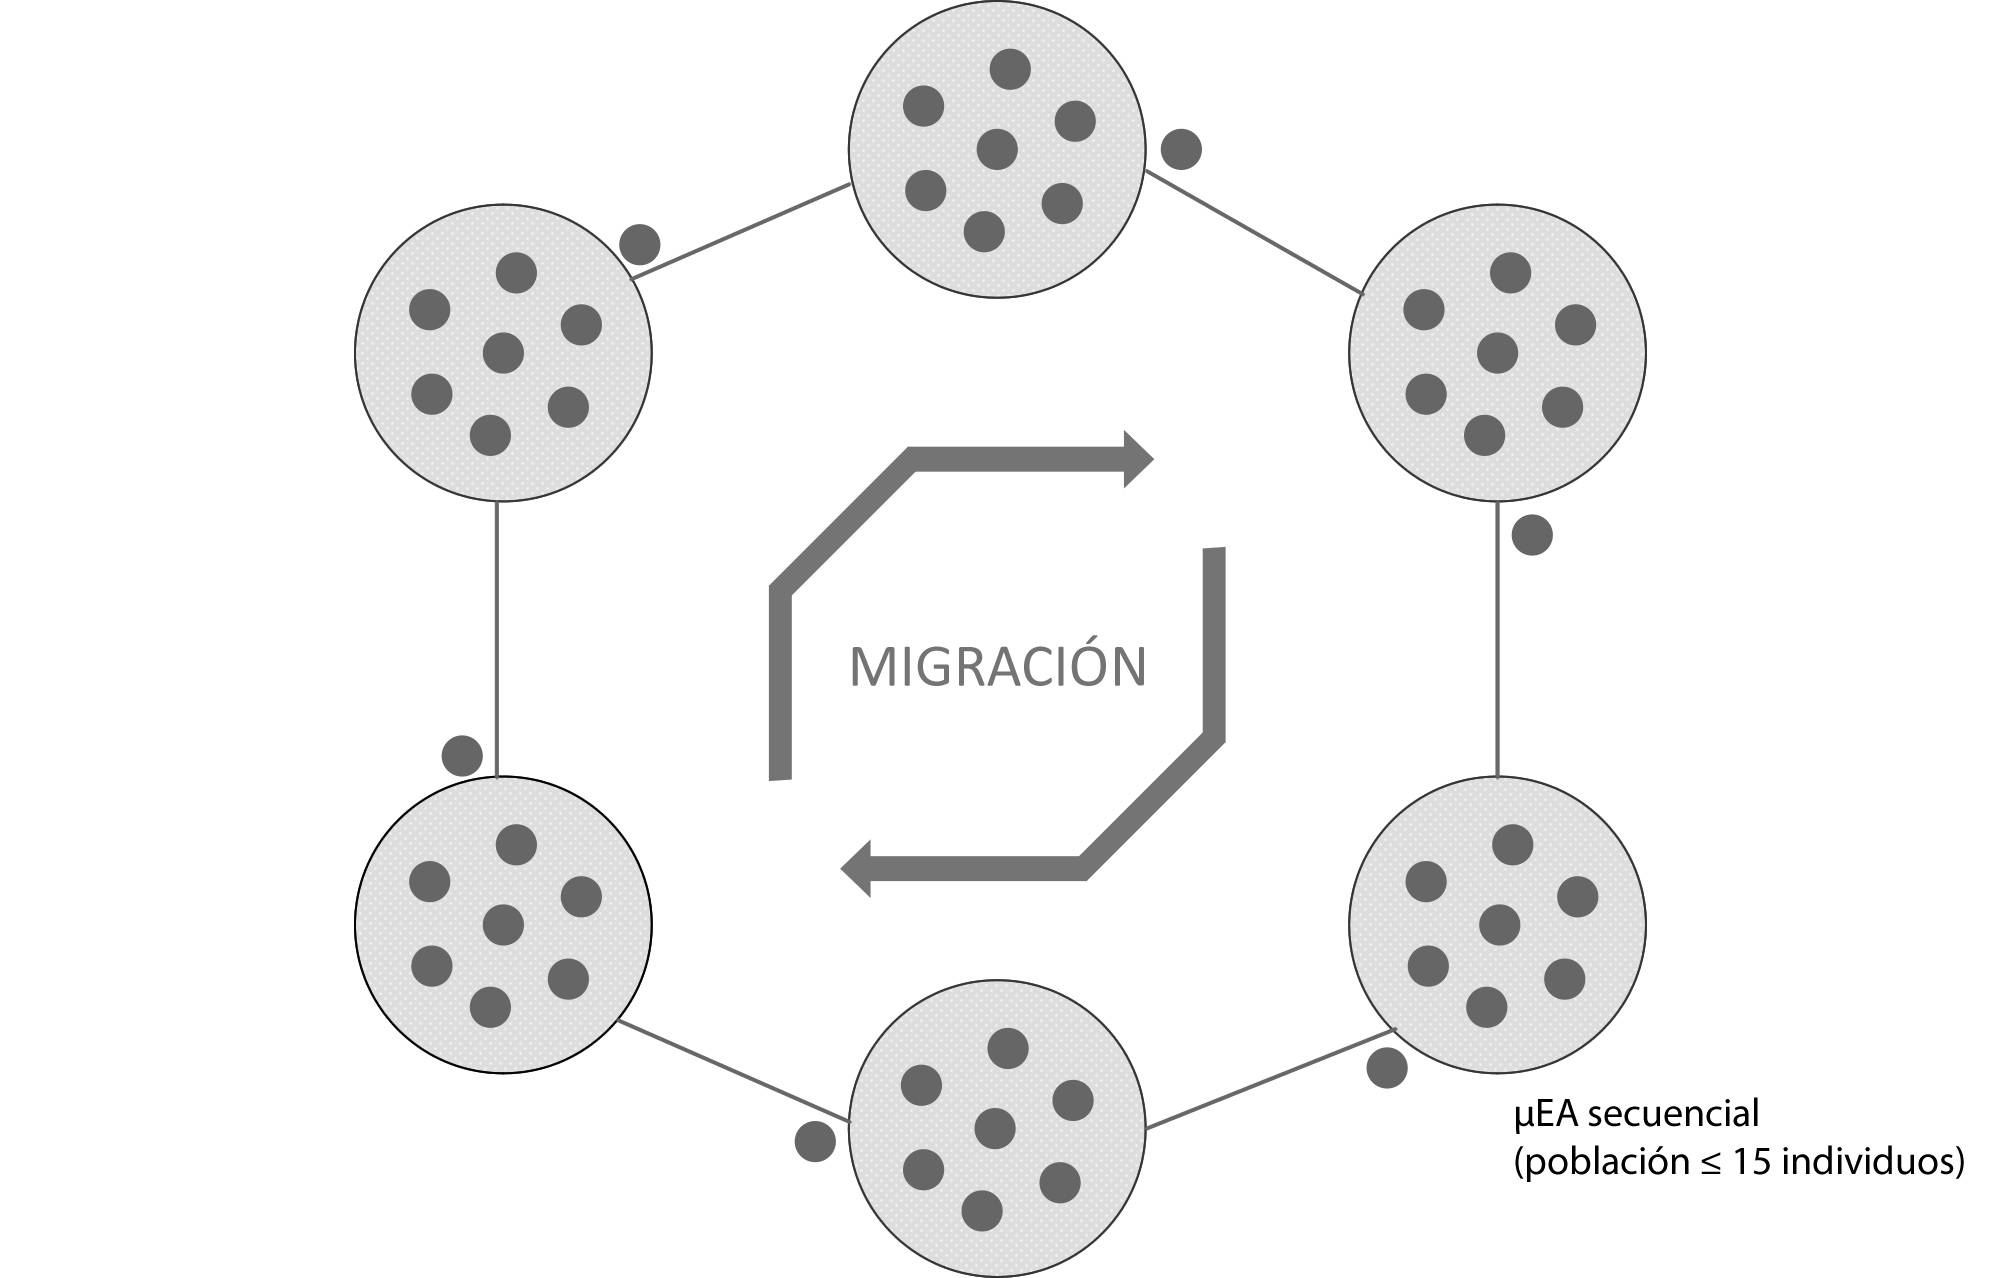
\includegraphics[width=1\textwidth]{migracion.png}}}}%
		\includegraphics<3->[width=1\textwidth]{migracion.png}
		%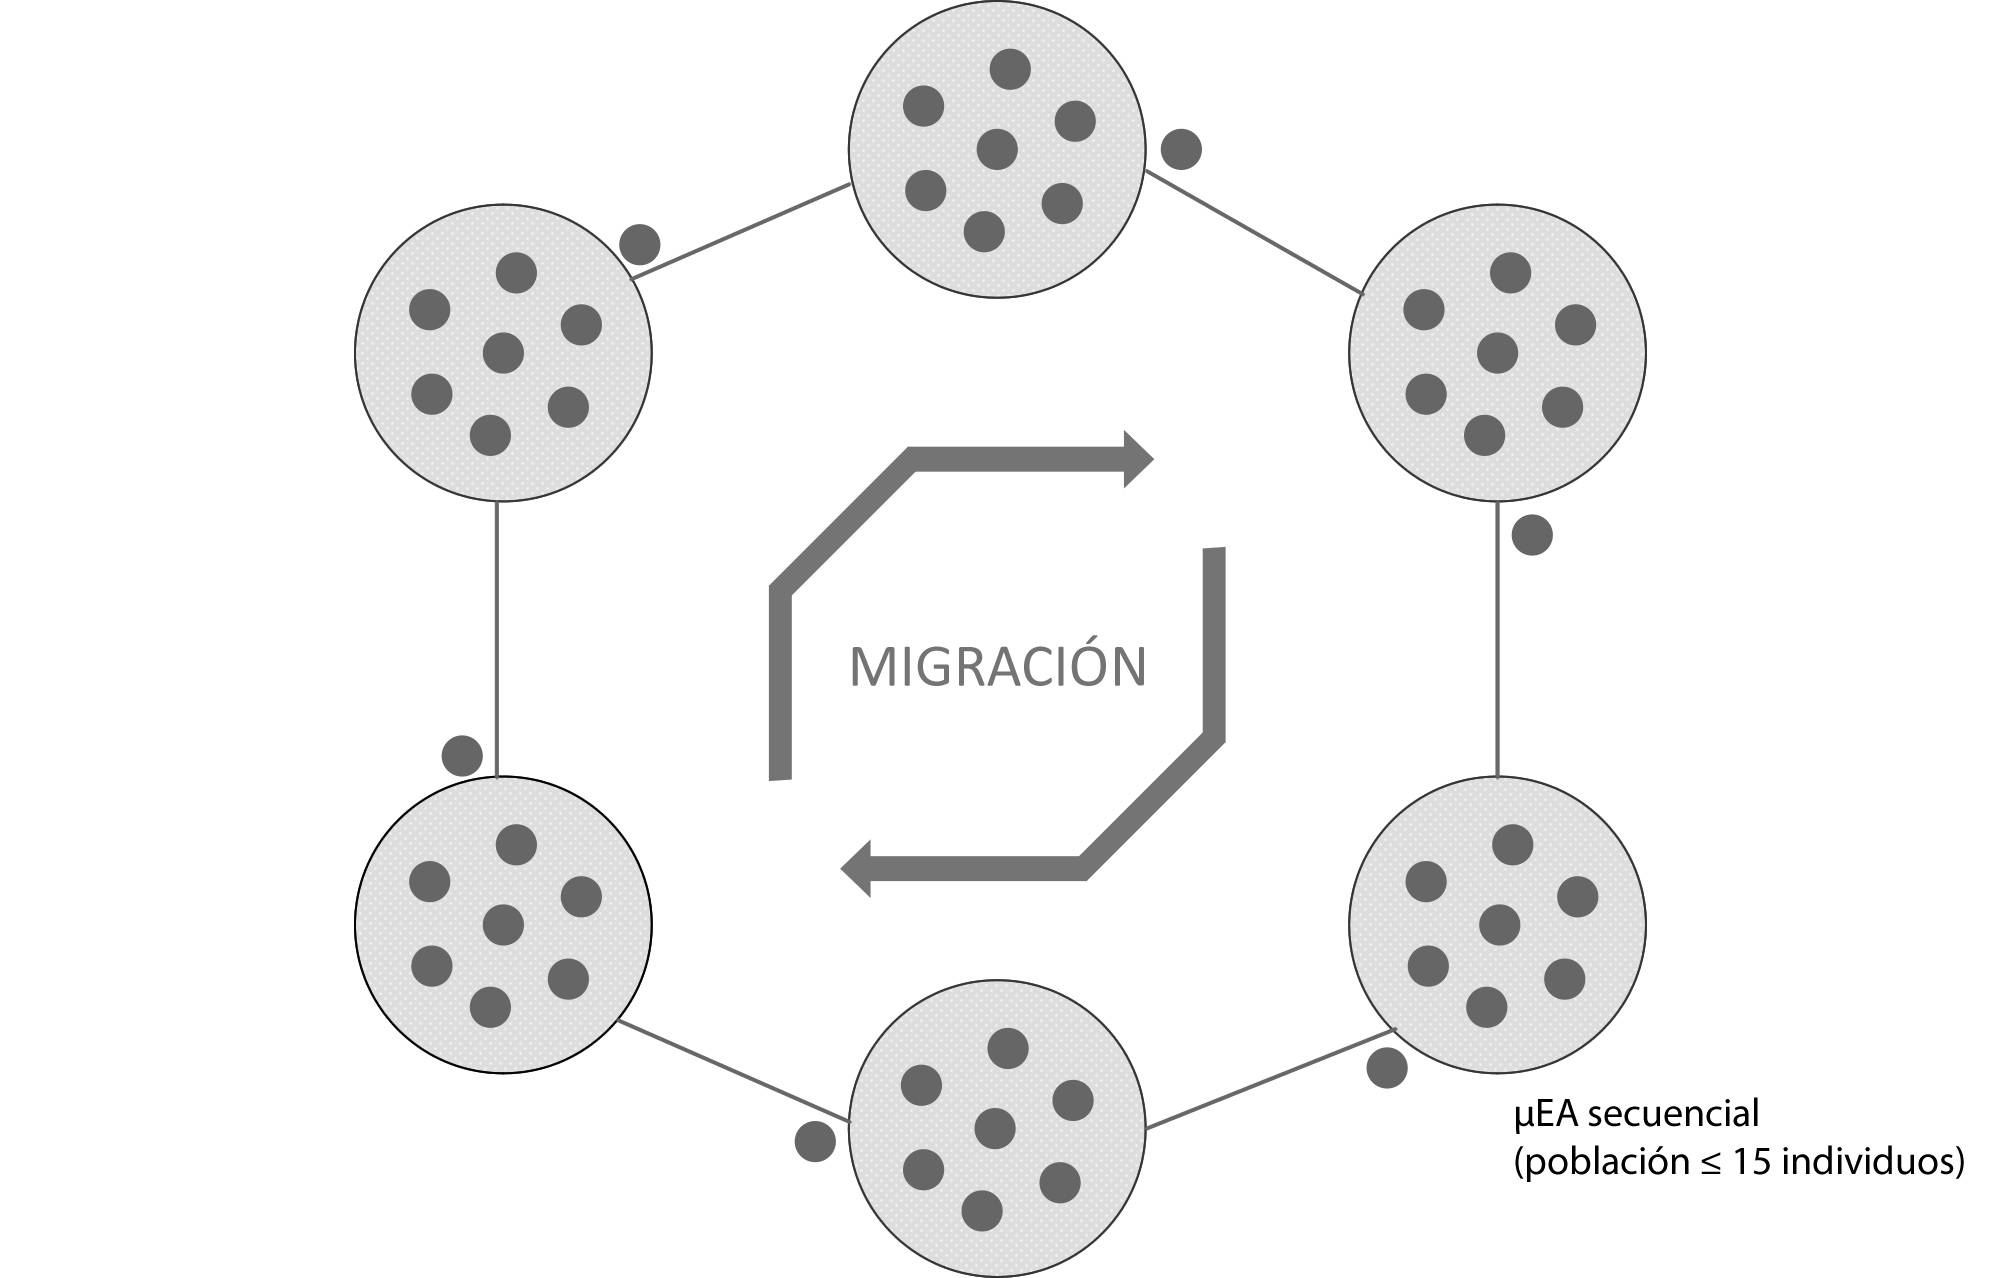
\includegraphics[width=.9\textwidth]{migracion.png}
	\end{columns}
}


\frame{
	\frametitle{AE para el PVCT multiobjetivo}
	\begin{block}{Propósitos en AE multiobjetivos (MOEA)}
			Acercarse al frente de Pareto del problema (\textbf{convergencia}) y muestrear adecuadamente el frente de soluciones (\textbf{diversidad}).
	\end{block}

	\pause
	\begin{columns}[totalwidth=\textwidth]
	\column{0.6\textwidth}
		\begin{block}{\textit{p$\mu$MOEA/D}}
		%Micro--poblaciones distribuidas con agregación lineal de los objetivos.
		$F = w_C\times CT + w_D \times DT$,\\\hspace{1cm} {\tiny$w_C = [0:\frac{1}{\#islas}:1]$, $w_D = 1 - w_C$}.
		\end{block}
	\column{0.4\textwidth}
		\centering
		\only<1>{\mbox{\phantom{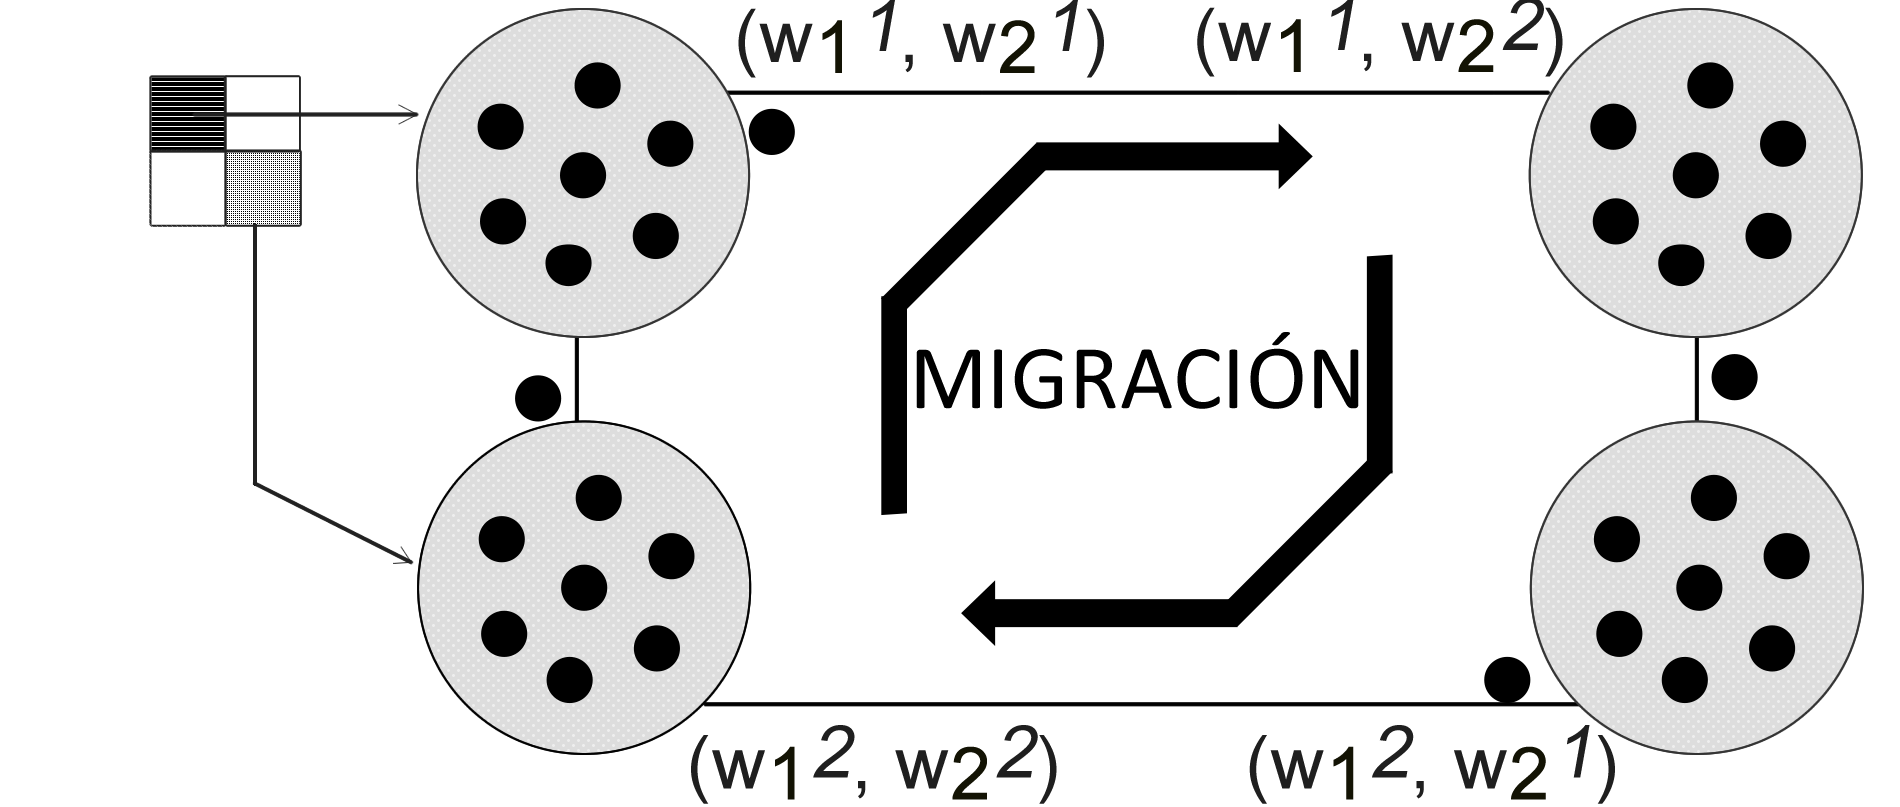
\includegraphics[width=0.9\textwidth]{pmuMOEAD.png}}}}%
		\includegraphics<2->[width=0.9\textwidth]{pmuMOEAD.png}
		%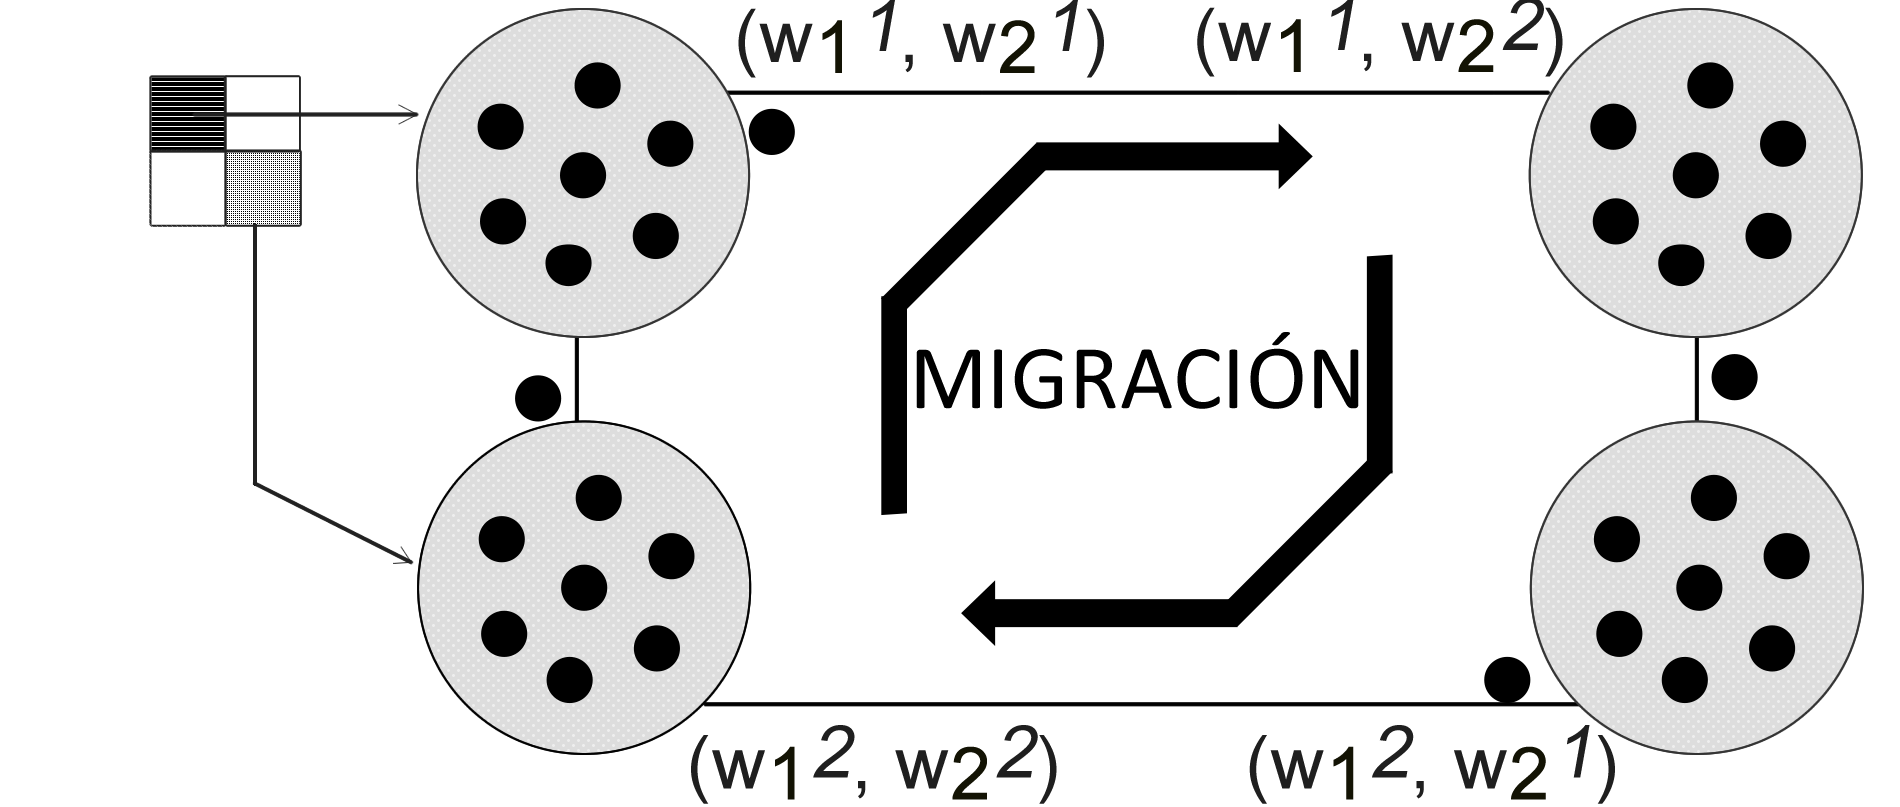
\includegraphics[width=.8\textwidth]{pmuMOEAD.png}
	\end{columns}
	\pause
	\begin{block}{\textit{NSGA--II}}
		Ordenamiento no--dominado (elitista) y \textit{crowding} para preservar diversidad.
	\end{block}
	\pause
	\begin{block}{Aspectos comunes}
		Función correctiva considera vehículos de distintas capacidades.
		Inicialización de la población ávida y selección por torneo.
	\end{block}\pause

}

% Slide - Evaluación Experimental ==============================================================
\section{Evaluación experimental} 
\frame{\tableofcontents[currentsection]}

\frame{
	\frametitle{Generación de instancias}
	
	\begin{block}{Generación de puntos realistas en el mapa}
		\begin{itemize}
		\item Generador de Pedidos de Taxis (TQG) con datos de GPS de taxis de Beijing (Ma et al., 2013).
		\item Script para obtener instancias de un origen a muchos destinos.
		\item Instancias en Montevideo generadas manualmente.
		\item API para obtener tarifas TaxiFareFinder (TFF).
		\end{itemize}
	\end{block}
	\pause
	\begin{block}{Instancias generadas}

	\begin{itemize}\setlength\itemsep{1pt}
		\item \textbf{6 chicas:} 10 y 15 pasajeros (Beijing).
		\item \textbf{6 medianas:} 15 y 25 pasajeros (Beijing).
		\item \textbf{6 grandes:} 25 y 45 pasajeros (Beijing).
		\item \textbf{4 en Montevideo:} 8 y 17 pasajeros (Montevideo).
	\end{itemize}
	
	\alert{22} instancias para el PVCT monoobjetivo, y un total de \alert{88} para el multiobjetivo, considerando distintas capacidades y tolerancias.
	
	\end{block}

}

\frame{
	\frametitle{PVCT monoobjetivo}
	\begin{block}{Entorno de ejecución}
		\begin{itemize}
		\item La evaluación experimental fue realizada en el Cluster FING.
		\item \textbf{seqEA}: Dell Power Edge 2950, \textbf{1 núcleo} de Intel Xeon E5430 2.66GHz, 8GB RAM.
		\item \textbf{p$\mu$EA}: HP Proliant DL585, \textbf{24 núcleos} de AMD Opteron 2.09GHz, 48GB RAM.
		\end{itemize}
	\end{block}
	\begin{block}{Configuración paramétrica}
	\begin{itemize}
		\item \textbf{seqEA}: 20 ejecuciones de 2000 generaciones sobre 3 instancias.\\{\small $\text{\#\textit{P}} \in \lbrace 150, 200, \alert{250}\rbrace$; $p_C \in \lbrace \alert{0.6}, 0.75, 0.95\rbrace$; $p_M \in \lbrace 0.001, 0.01, \alert{0.1}\rbrace$.}\\
	
		\item \textbf{p$\mu$EA}: micro--población de 15 individuos, torneo ($m=2$, $k=1$), migración cada 500 generaciones. \\20 ejecuciones de 100.000 generaciones sobre 5 instancias.\\{\small $p_C \in \lbrace 0.6, \alert{0.75}, 0.95\rbrace$; $p_M \in \lbrace 0.001, 0.01, \alert{0.1}\rbrace$.}
	\end{itemize}
	\end{block}

}

\frame{	
	\frametitle{Algoritmo ávido}
	Utiliza ideas de los trabajos relacionados. Toma \textbf{decisiones localmente óptimas} y emula el comportamiento de un grupo de usuarios humanos.
	\includegraphics[width=1.\linewidth]<1>{greedy_costo_1}
	\includegraphics[width=1.\linewidth]<2>{greedy_costo_2}
	\includegraphics[width=1.\linewidth]<3>{greedy_costo_3}
	\includegraphics[width=1.\linewidth]<4>{greedy_costo_4}
	\includegraphics[width=1.\linewidth]<5>{greedy_costo_5}
	\includegraphics[width=1.\linewidth]<6>{greedy_costo_6}
	\includegraphics[width=1.\linewidth]<7>{greedy_costo_7}
	\includegraphics[width=1.\linewidth]<8>{greedy_costo_8}

}

\frame{
	\frametitle{Comparativa de métodos de inicialización}
	\begin{block}{Metodología}
		\begin{itemize}
			\item Shapiro--Wilk afirma que los resultados no siguen una distribución normal.
			\item Se utilizó Kruskal--Wallis para comparar ambas inicializaciones.
			\item Kruskal--Wallis permite afirmar con un nivel de confianza del 95\% que una de las inicializaciones obtuvo mejores resultados que la otra.
		\end{itemize}
	\end{block}
	
	\begin{block}{\textit{seqEA} con inicialización aleatoria vs. incialización ávida}
		La inicialización ávida supera a la inicialización aleatoria en \alert{10} instancias de prueba, mientras que la inicialización aleatoria lo hace en tan solo \alert{2}.
	\end{block}
	
	\begin{block}{\textit{p$\mu$EA} con inicialización aleatoria vs. incialización ávida}
		La inicialización ávida super a la inicialización aleatoria en \alert{11} instancias de prueba, mientras que no hubo instancias en las que se pueda afirmar que la inicialización aleatoria haya alcanzado mejores soluciones.
	\end{block}
}

\frame{
	\frametitle{Mejora \textit{seqEA} sobre algoritmo ávido}
	Se alcanzaron mejores valores en \textbf{todas} las instancias. En el mejor caso se superó el costo del algoritmo ávido en un \alert{35.9\%}.
	\begin{columns}[t]
\column{.5\textwidth}
\centering
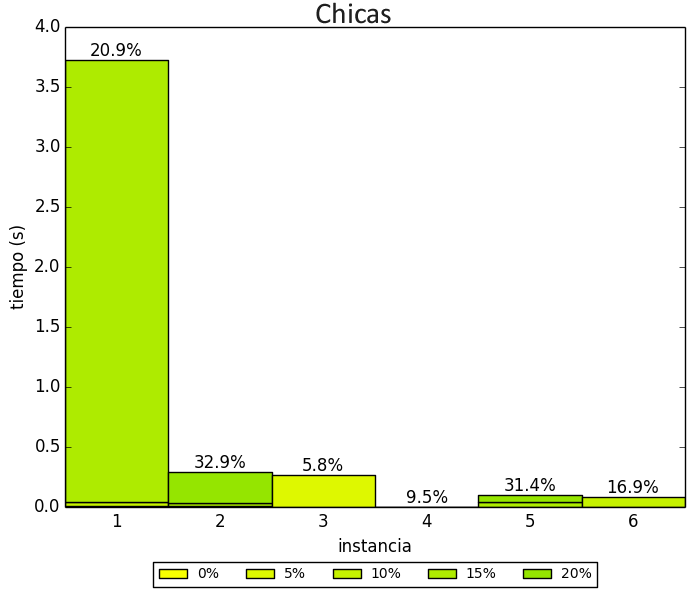
\includegraphics[width=4.5cm,height=3.5cm]{./evaluacion_experimental/mejoras_greedy_clei/greedy_costo_Chicas}\\
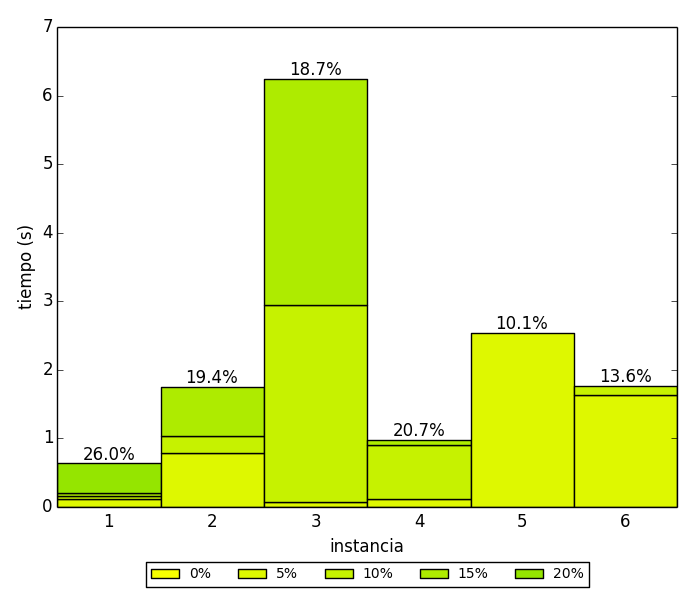
\includegraphics[width=4.5cm,height=3.5cm]{./evaluacion_experimental/mejoras_greedy_clei/greedy_costo_Medianas}
\column{.5\textwidth}
\centering
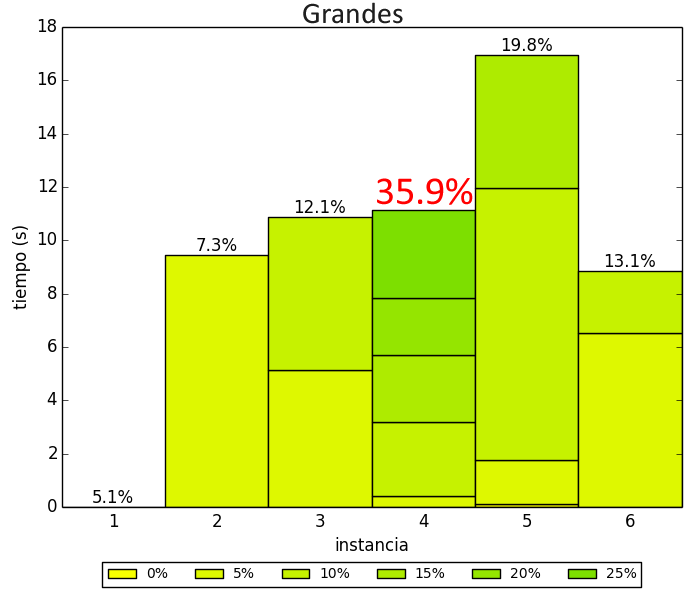
\includegraphics[width=4.5cm,height=3.5cm]{./evaluacion_experimental/mejoras_greedy_clei/greedy_costo_Grandes}\\
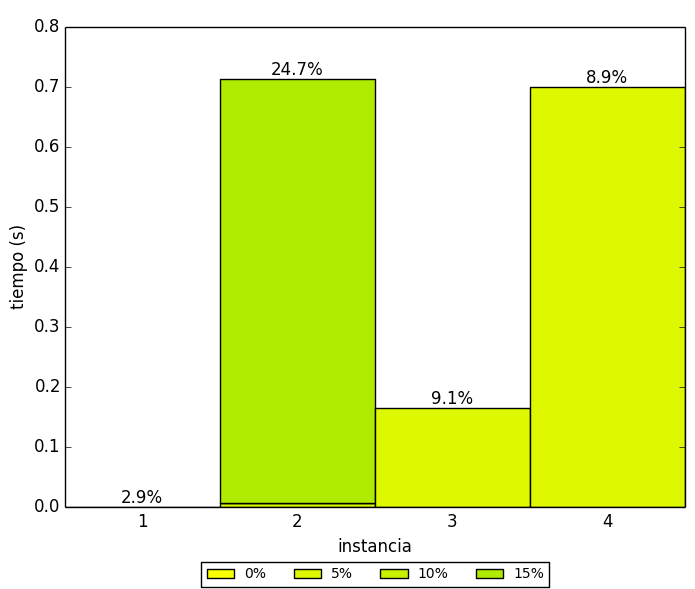
\includegraphics[width=4.5cm,height=3.5cm]{./evaluacion_experimental/mejoras_greedy_clei/greedy_costo_Montevideo}
\end{columns}
}

\frame{
	\frametitle{Mejora \textit{p$\mu$EA} sobre algoritmo ávido}
	Se alcanzaron mejores valores en \textbf{todas} las instancias. En el mejor caso se superó el costo del algoritmo ávido en un \alert{41.0\%}.
	\centering
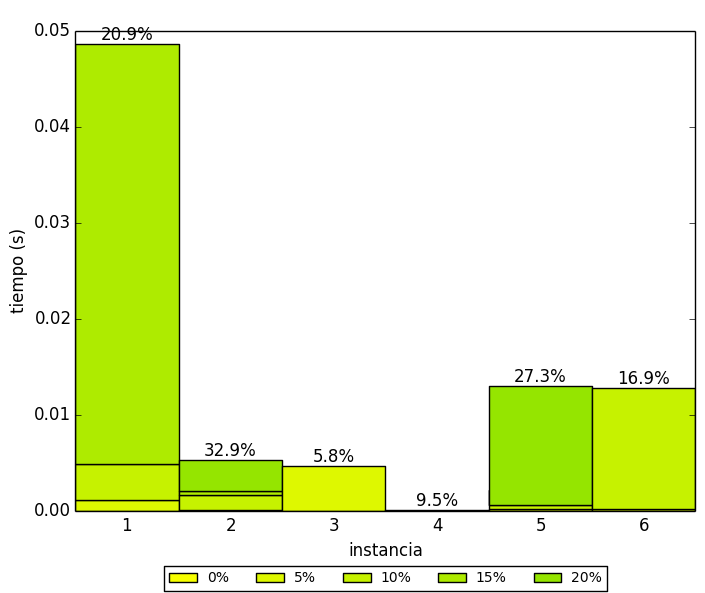
\includegraphics[width=9cm,height=7cm]{./evaluacion_experimental/mejoras_greedy_alio/greedy_costo_Chicas}\\
}

\frame{
	\frametitle{Comparativa \textit{seqEA} vs. \textit{p$\mu$EA}}
	Sobre un total de 22 instancias, \textit{p$\mu$EA} es capaz de encontrar mejores resultados que \textit{seqEA} en \alert{17}. Únicamente en \alert{1} instancia de prueba \textit{seqEA} alcanzó mejores soluciones que \textit{p$\mu$EA}.
	
	\vspace{0.15cm}
	
	\centering
\begin{adjustbox}{max width=0.55\textwidth}
\begin{tabular}{ccrrrrr}
\multicolumn {2}  {c} {\multirow{2}{*}{\textit{instancia}}}  & \multicolumn {2}  {c} {\textit{seqEA}} &\multicolumn {2}  {c}{\textit{p$\mu$EA}} &\multirow {2}  {*}{\textit{pvK--W}}\\
	   & 	&\multicolumn {1}  {c}{$min(c)$}	& \multicolumn {1}  {c}{$\overline{c}\pm std$}	& \multicolumn {1}  {c}{$min(c)$} &\multicolumn {1}  {c}{$\overline{c}\pm std$}	& \\
\midrule
\multirow {6}  {*} {chicas}     	& \#1             	& 164.4  				& 165.6$\pm$2.0                		& 164.4 & \alert{164.4}$\alert{\pm}$\alert{0.0}        & 0.2$\times 10^{-3}$   \\
                                		& \#2             	& 220.7  				& 225.7$\pm$5.0                		& 220.7 & \alert{220.7}$\alert{\pm}$\alert{0.0}        & 9.7$\times 10^{-6}$   \\
                                		& \#3             	& 160.4  				& 160.4$\pm$0.0                		& 160.4 & 160.4$\pm$0.0         & 1.0                 \\
                                		& \#4             	& 181.3  				& 181.3$\pm$0.1       			& 181.3 & 182.4$\pm$1.9       & 0.5$\times 10^{-1}$     \\
                                		& \#5             	& 152.1  				& 155.6$\pm$4.5                		& 152.1 & \alert{152.1}$\alert{\pm}$\alert{0.0}        & 5.1$\times 10^{-6}$   \\
                                		& \#6             	& 118.4  				& 119.6$\pm$2.5                		& 118.4 & \alert{118.4}$\alert{\pm}$\alert{0.0}        & 0.1$\times 10^{-1}$     \\
\hline
\multirow {6}  {*} {medianas}   	& \#1             	& 211.9 				& 216.0$\pm$4.2                 		& 211.9 & \alert{211.9}$\alert{\pm}$\alert{0.0}        & 5.2$\times 10^{-11}$   \\
                                		& \#2             	& 428.6 				& 444.1$\pm$11.7                		& 427.9 & \alert{429.4}$\alert{\pm}$\alert{1.6}        & 7.0$\times 10^{-10}$  \\
                               		 	& \#3             	& 361.7 				& 378.7$\pm$6.5                 		& 364.5 & \alert{370.4}$\alert{\pm}$\alert{4.5}        & 1.6$\times 10^{-6}$   \\
                                		& \#4             	& 267.5 				& 279.8$\pm$5.5                 		& 266.8 & \alert{266.8}$\alert{\pm}$\alert{0.0}        & 7.6$\times 10^{-12}$   \\
                               	 		& \#5             	& 479.3 				& 487.1$\pm$6.5                 		& 479.6 & \alert{479.8}$\alert{\pm}$\alert{0.2}        & 5.1$\times 10^{-7}$   \\
                                		& \#6             	& 306.0 				& 321.2$\pm$7.7                 		& 306.0 & \alert{307.7}$\alert{\pm}$\alert{3.4}        & 2.0$\times 10^{-9}$   \\
\hline
\multirow {6}  {*} {grandes}    	& \#1             	& 421.9 				& \alert{435.1}$\alert{\pm}$\alert{5.0}        		& 425.9 & 437.7$\pm$3.2       & 0.1$\times 10^{-1}$     \\
                                		& \#2             	& 479.3 				& 489.9$\pm$4.3                 		& 477.0 & \alert{481.1}$\alert{\pm}$\alert{2.3}        & 1.9$\times 10^{-9}$   \\
                                		& \#3             	& 332.8 				& 349.7$\pm$7.7                 		& 326.3 & \alert{331.7}$\alert{\pm}$\alert{4.0}        & 2.6$\times 10^{-10}$  \\
                                		& \#4             	& 351.1 				& 390.7$\pm$26.3                		& 338.4 & \alert{344.8}$\alert{\pm}$\alert{6.1}        & 5.1$\times 10^{-11}$   \\
                                		& \#5             	& 395.9 				& 429.6$\pm$16.2                		& 370.2 & \alert{380.0}$\alert{\pm}$\alert{4.4}        & 2.7$\times 10^{-11}$   \\
                                		& \#6             	& 360.8 				& 382.4$\pm$8.1                 		& 343.8 & \alert{350.6}$\alert{\pm}$\alert{3.8}        & 2.6$\times 10^{-11}$   \\
\hline
\multirow {4}  {*} {Montevideo} & \#1            	& 168.4 				& 168.4$\pm$0.0                 		& 168.4 & 168.4$\pm$0.0         & 1.0                 \\
                                		& \#2            	& 319.3 				& 331.2$\pm$3.8                 		& 324.9 & \alert{328.6}$\alert{\pm}$\alert{3.2}        & 5.6$\times 10^{-6}$   \\
                                		& \#3             	& 266.7 				& 269.1$\pm$2.3                 		& 266.7 & \alert{266.7}$\alert{\pm}$\alert{0.0}        & 3.1$\times 10^{-7}$   \\
                                		& \#4             	& 303.2 				& 304.7$\pm$0.5                 		& 304.1 & 304.5$\pm$0.4         & 0.1       \\\bottomrule
\end{tabular}
\end{adjustbox}


}

\frame{
	\frametitle{Evolución del costo a lo largo de la ejecución}
	\textit{p$\mu$EA} alcanza mejores soluciones que \textit{seqEA} en menos tiempo. En el mejor caso la aceleración es de $7.5$x ($4.6$x en promedio).
	
	\begin{columns}[t]
\column{.5\textwidth}
\centering
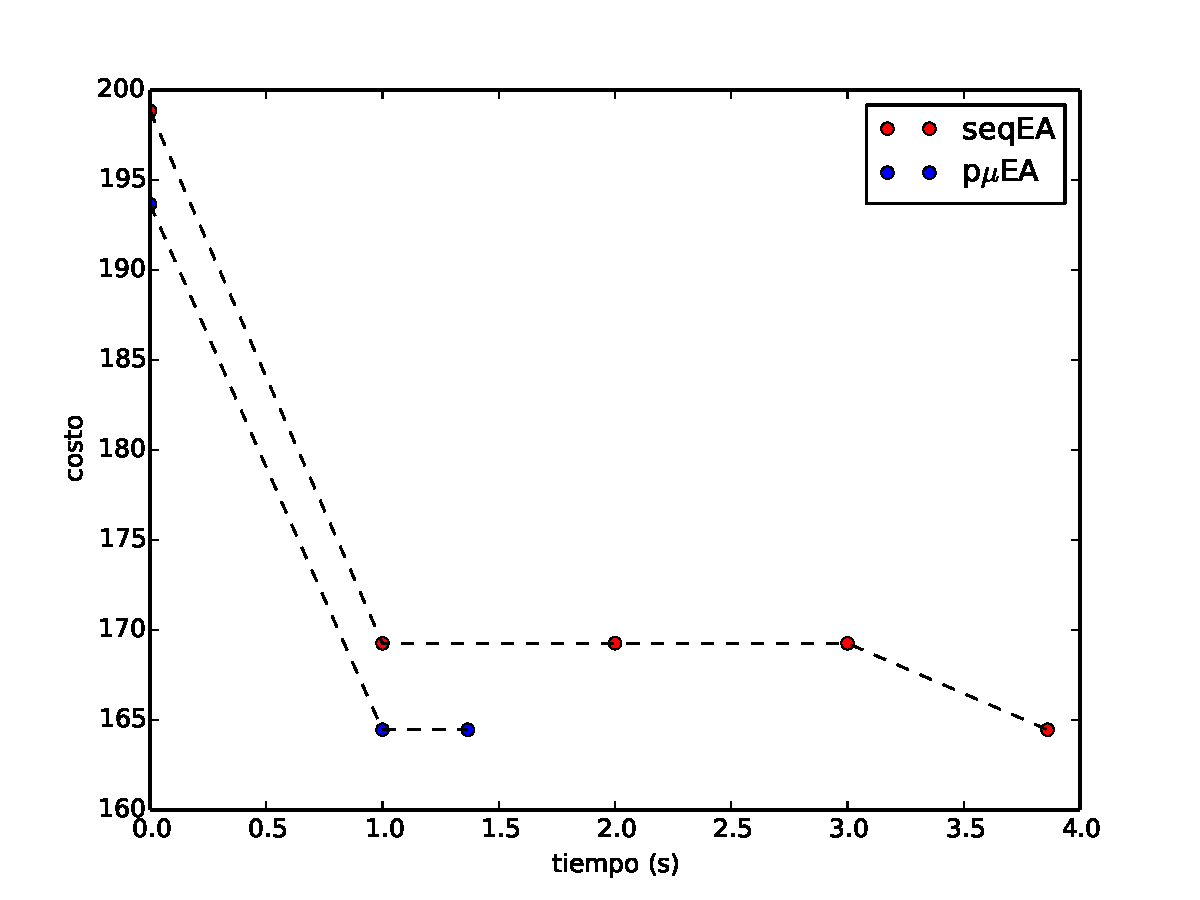
\includegraphics[width=4.5cm,height=3.5cm]{./evaluacion_experimental/fitness_sobre_tiempo/chicas_1.pdf}\\
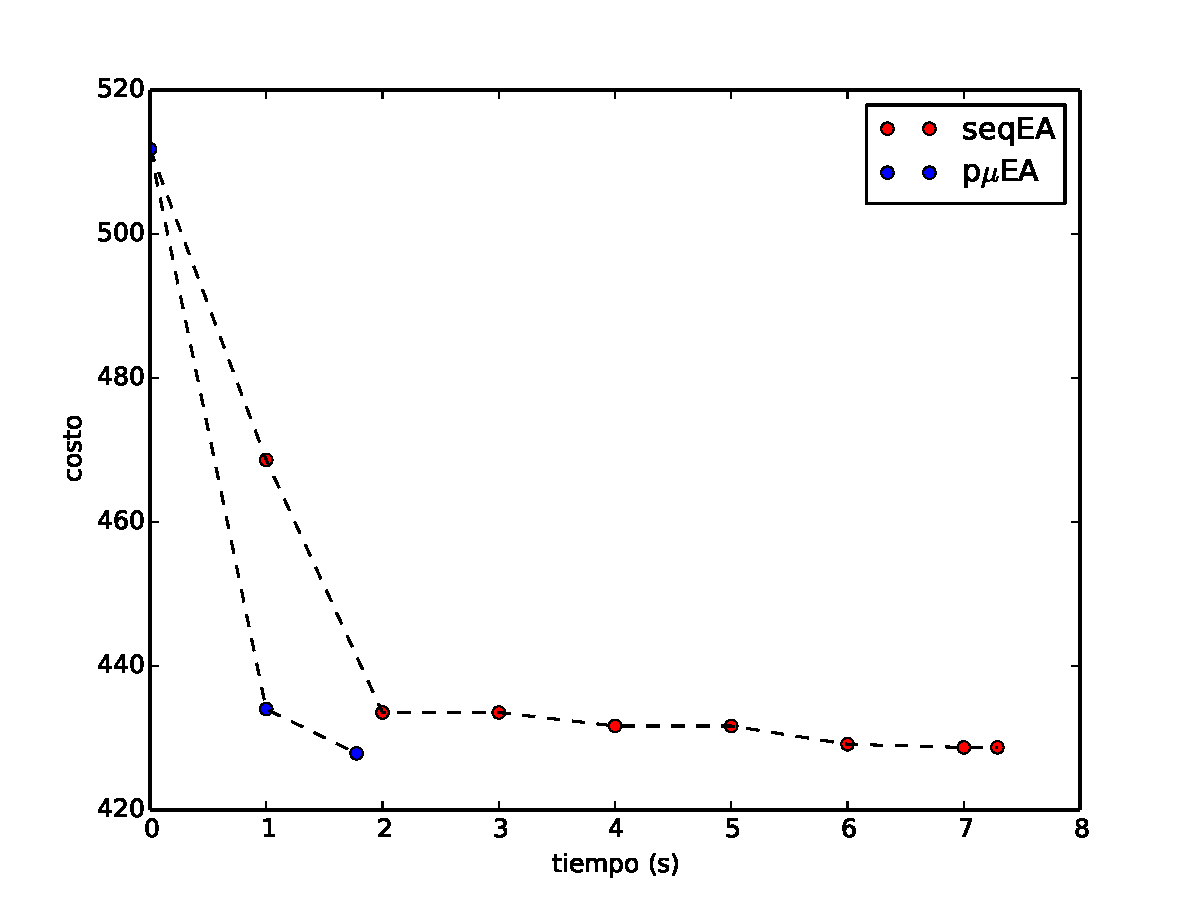
\includegraphics[width=4.5cm,height=3.5cm]{./evaluacion_experimental/fitness_sobre_tiempo/medianas_2.pdf}
\column{.5\textwidth}
\centering
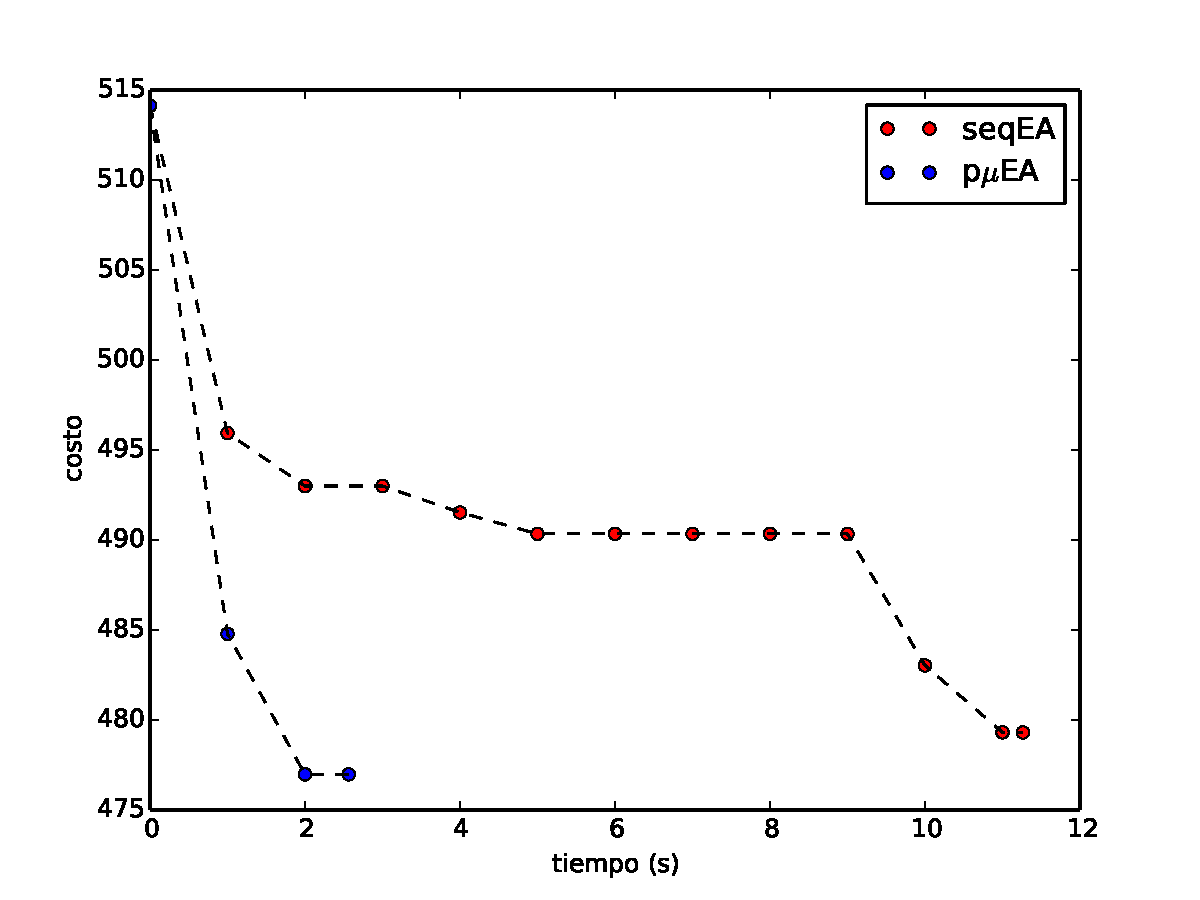
\includegraphics[width=4.5cm,height=3.5cm]{./evaluacion_experimental/fitness_sobre_tiempo/grandes_2.pdf}\\
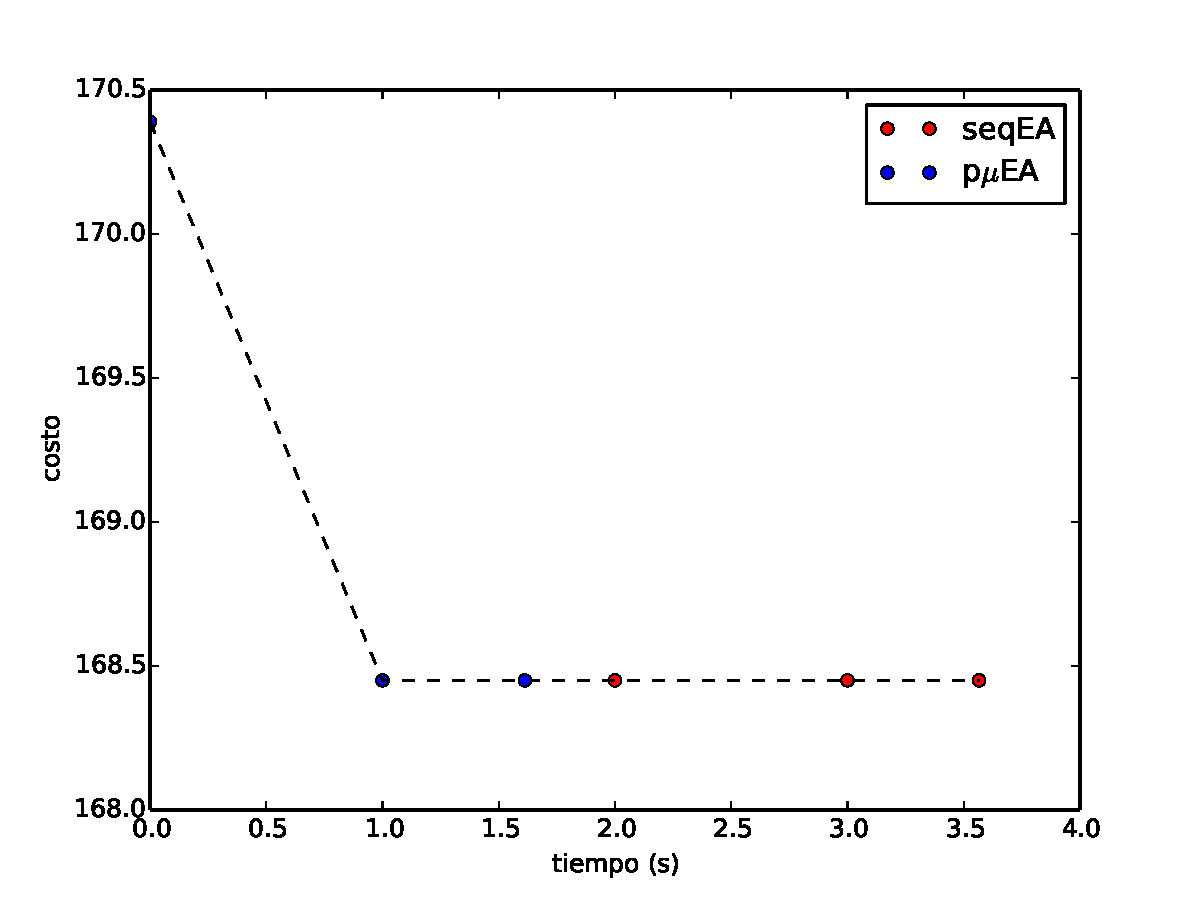
\includegraphics[width=4.5cm,height=3.5cm]{./evaluacion_experimental/fitness_sobre_tiempo/montevideo_1.pdf}
\end{columns}
}

\frame{
	\frametitle{PVCT multiobjetivo}

	\begin{block}{Entorno de ejecución}
		\begin{itemize}
			\item La evaluación experimental fue realizada en el Cluster FING.
			\item \textbf{p$\mu$MOEA/D}: HP Proliant DL585, \textbf{24 núcleos} de AMD Opteron 2.09GHz, 48GB RAM.
			\item \textbf{NSGA--II}: HP Proliant DL385 G7, \textbf{1 núcleo} de AMD Opteron 6172 2.10GHz, 72GB RAM.
		\end{itemize}
	\end{block}
	
	\begin{block}{Configuración paramétrica}
		\begin{itemize}
			\item \textbf{p$\mu$MOEA/D}: 30 ejecuciones de 20000 generaciones sobre 4 instancias. \\{\small $P=15$; $p_C \in \lbrace 0.6, \alert{0.75}, 0.95\rbrace$; $p_M \in \lbrace 0.001, 0.01, \alert{0.1}\rbrace$; operador de migración cada 1000 generaciones.}\\
			\item \textbf{NSGA--II}: 30 ejecuciones de 5000 generaciones sobre 4 instancias. \\{\small $P=80$; $p_C \in \lbrace 0.6, \alert{0.75}, 0.95\rbrace$; $p_M \in \lbrace 0.001, 0.01, \alert{0.1}\rbrace$.}\\
		\end{itemize}
	\end{block}
}

\frame{
	\frametitle{Algoritmos ávidos}
	
	\begin{block}{Algoritmo ávido para minimizar el costo}
		Se utilizó el mismo algoritmo detallado previamente, tomando en cuenta las distintas capacidades de los vehículos y su disponibilidad.
	\end{block}

	\begin{block}{Algoritmo ávido para minimizar la demora}
		\begin{itemize}
		\item En primera instancia, se crea un taxi vacío para cada uno de los pasajeros con mayor nivel de apuro. 
		\item Se ubica a cada pasajero con mayor nivel de apuro en la primera posición del taxi.
		\item Luego, se recorre la lista de pasajeros no asignados en orden de apuro, colocándolos en el taxi que minimice su demora.
		\item Si el taxi completa la máxima capacidad disponible, se lo considera \textit{completo} y no acepta más pasajeros.
		\end{itemize}
	\end{block}
}

\frame{
	\frametitle{Métricas multiobjetivo}
		
	\begin{block}{\textit{p$\mu$MOEA/D}}
		Se logra una buena convergencia y diversidad. Sin embargo, la cantidad de soluciones no dominadas es baja, indicando que se puede mejorar.

		%La baja distancia generacional y el spread indican buena convergencia y diversidad. El hipervolumen refuerza estas afirmaciones, aunque la cantidad de soluciones no dominadas resulta baja.

		\centering
\begin{adjustbox}{max width=1\textwidth}
\begin{footnotesize}
\begin{tabular}{lrrrrr}
\toprule
			&\multicolumn{1}{c}{\#ND}& \multicolumn{1}{c}{DG} & \multicolumn{1}{c}{spacing} & \multicolumn{1}{c}{spread} & \multicolumn{1}{c}{RHV} \\\midrule
 chicas     & 8.5$\pm$2.1 (16.0) & 3.1$\pm$2.5 (0.0) & 740.2$\pm$746.3 (58.1)    & 0.6$\pm$0.2 (0.1) & 0.9$\pm$0.1 (1.0) \\
 medianas   & 9.1$\pm$2.2 (19.0) & 5.7$\pm$2.5 (0.0) & 1448.5$\pm$1064.1 (141.6) & 0.6$\pm$0.1 (0.1) & 0.9$\pm$0.1 (1.0) \\
 grandes   & 8.5$\pm$2.2 (17.0) & 7.9$\pm$3.4 (2.0) & 2917.2$\pm$2041.5 (175.3) & 0.6$\pm$0.1 (0.0) & 0.8$\pm$0.1 (1.0) \\
 Montevideo & 8.0$\pm$2.1 (14.0) & 3.0$\pm$2.0 (0.0) & 663.5$\pm$542.4 (61.5)    & 0.6$\pm$0.2 (0.0) & 0.9$\pm$0.0 (1.0) \\
\bottomrule
\end{tabular}
\end{footnotesize}
\end{adjustbox}
	\end{block}

	\begin{block}{\textit{NSGA--II}}
		La cantidad de puntos no dominados es mayor. La distancia generacional indica una buena convergencia y se logra una mayor dispersión.
	
		\begin{adjustbox}{max width=1\textwidth}
\centering
\begin{footnotesize}
\begin{tabular}{lrrrrr}
\toprule
			&\multicolumn{1}{c}{\#ND}& \multicolumn{1}{c}{DG} & \multicolumn{1}{c}{spacing} & \multicolumn{1}{c}{spread} & \multicolumn{1}{c}{RHV} \\\midrule

 chicas     & 32.6$\pm$9.5 (55.0)  & 0.3$\pm$0.6 (0.0) & 236.2$\pm$222.7 (43.2) & 0.9$\pm$0.1 (0.7) & 1.0$\pm$0.0 (1.0) \\
 medianas   & 54.5$\pm$4.2 (67.0)  & 1.0$\pm$0.7 (0.0) & 193.6$\pm$202.4 (26.2) & 0.7$\pm$0.2 (0.4) & 1.0$\pm$0.0 (1.0) \\
 grandes    & 55.2$\pm$3.5 (67.0)  & 1.8$\pm$1.1 (0.4) & 243.6$\pm$229.8 (26.4) & 0.7$\pm$0.2 (0.4) & 1.0$\pm$0.0 (1.0) \\
 Montevideo & 43.9$\pm$16.4 (61.0) & 0.4$\pm$0.5 (0.0) & 142.3$\pm$143.2 (20.8) & 0.8$\pm$0.1 (0.5) & 1.0$\pm$0.0 (1.0) \\

\bottomrule
\end{tabular}
\end{footnotesize}
\end{adjustbox}
	\end{block}	
	
}

\frame{
	\frametitle{Mejora frente a algoritmos ávidos vs. tiempo de ejecución}
	El enfoque multiobjetivo explícito de \textit{NSGA--II} permite alcanzar mejores resultados que el enfoque por descomposición de dominio aplicado en \textit{p$\mu$MOEA/D}. Sin embargo, los tiempos de ejecución son significativamente mayores.

	\begin{columns}[t]
	\column{.5\textwidth}
	\centering
		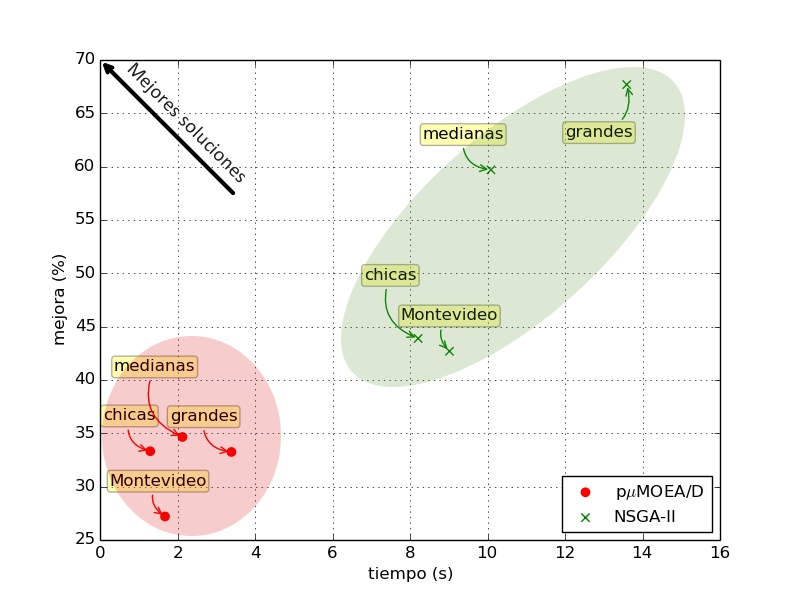
\includegraphics[width=6.075cm,height=4.725cm]{./evaluacion_experimental/tradeoff_maeb_mic/costo}\\
		\small \textit{costo}
	\column{.5\textwidth}
	\centering
		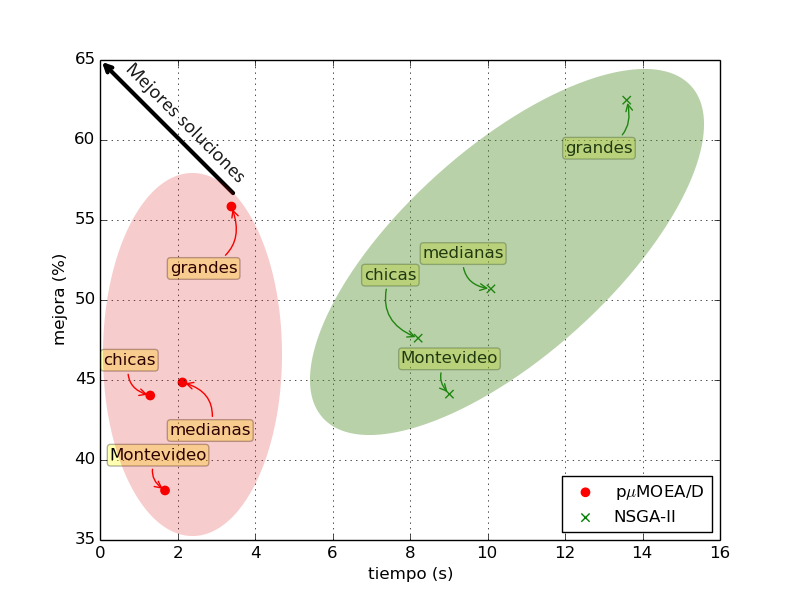
\includegraphics[width=6.075cm,height=4.725cm]{./evaluacion_experimental/tradeoff_maeb_mic/demora}\\
		\small \textit{demora}
\end{columns}
	
}

\frame{
	\frametitle{Frentes de Pareto: p$\mu$MOEA/D vs. NSGA--II}
	\alert{\textit{NSGA--II} alcanza mejores soluciones} con una mayor cantidad de puntos no dominados distribuidos homogéneamente a lo largo del frente.
	
	\begin{columns}[t]
\column{.5\textwidth}
\centering
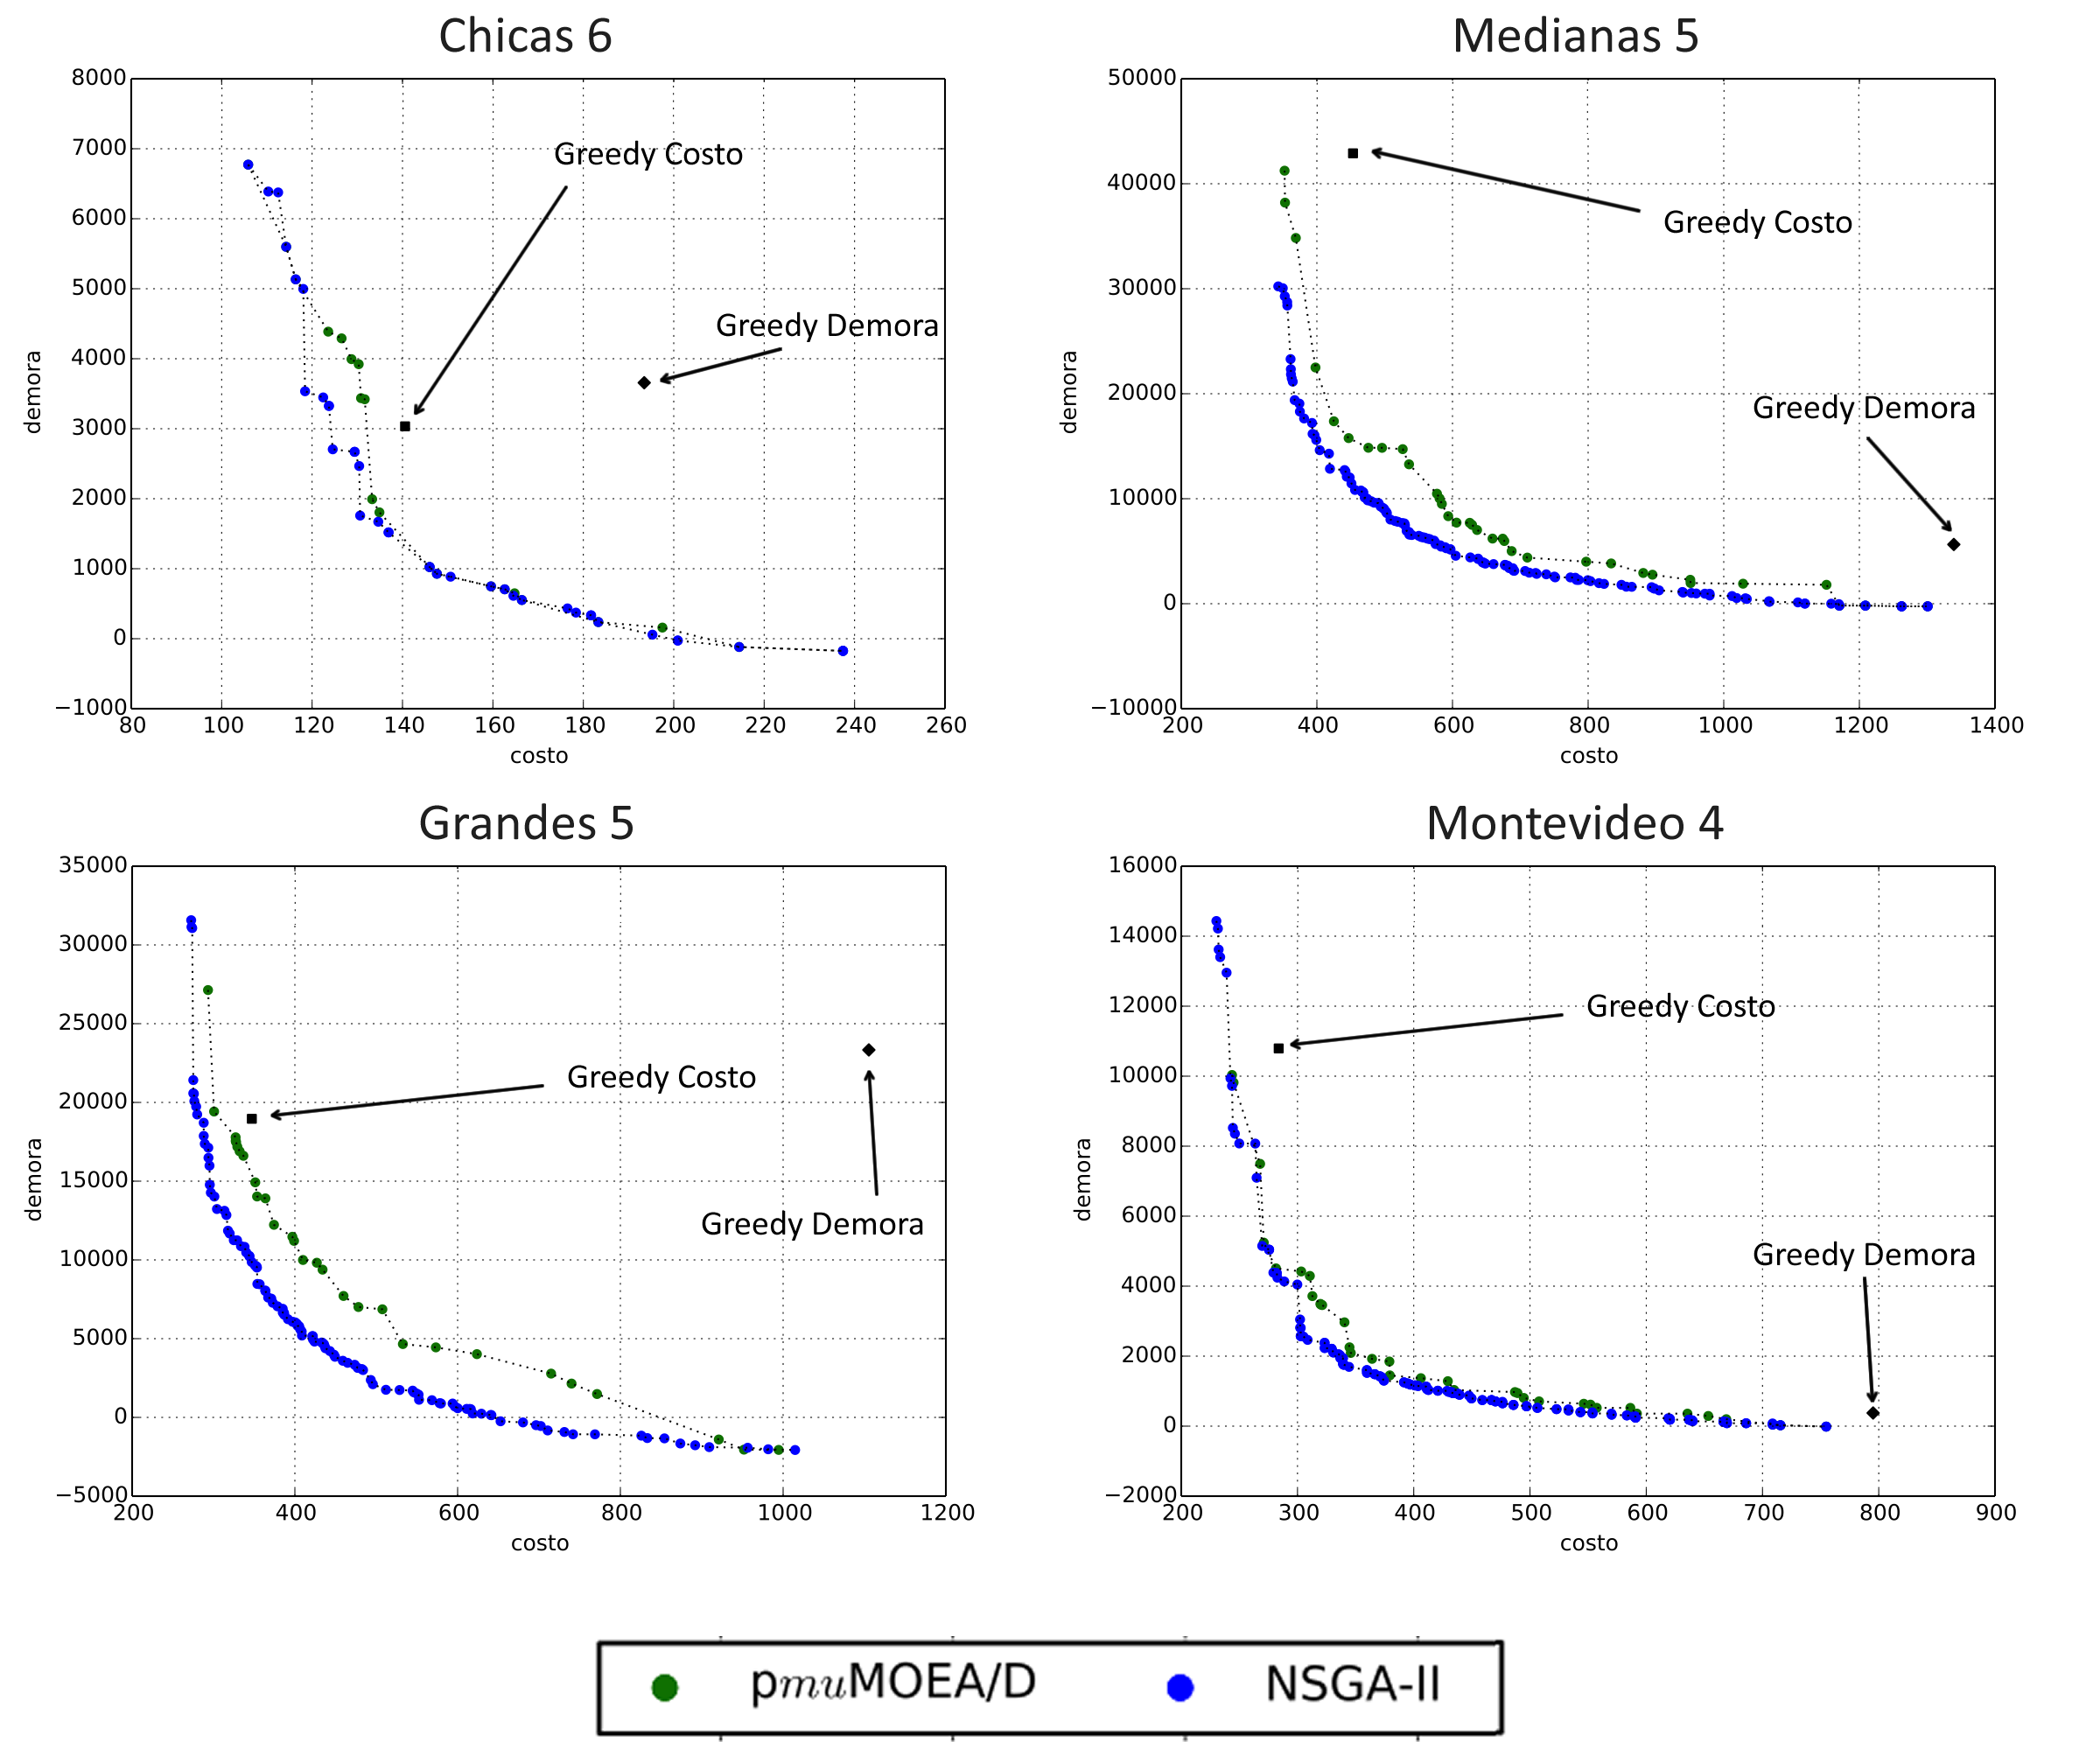
\includegraphics[width=4.5cm,height=3.5cm]{./evaluacion_experimental/fp_comparacion/Ch_6_1.png}\\
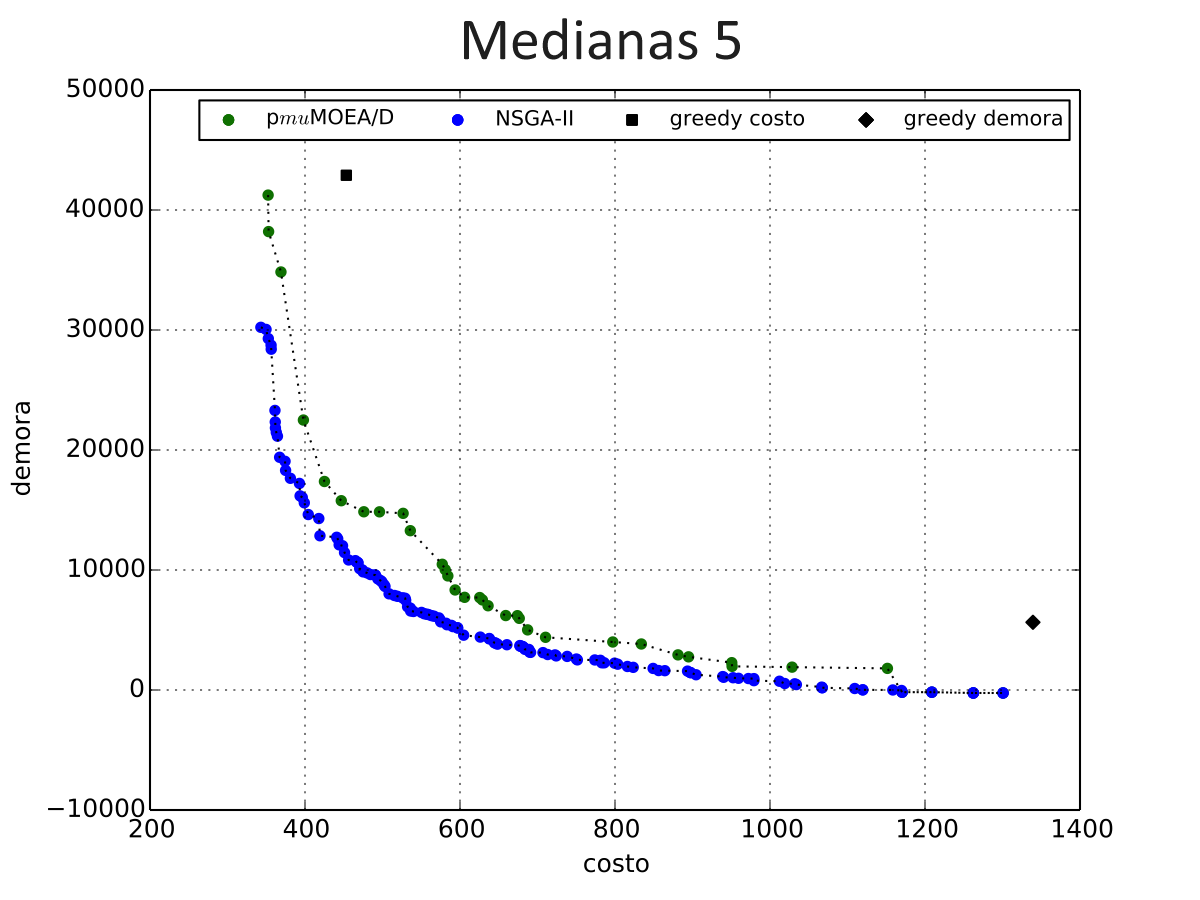
\includegraphics[width=4.5cm,height=3.5cm]{./evaluacion_experimental/fp_comparacion/Me_5_3.png}
\column{.5\textwidth}
\centering
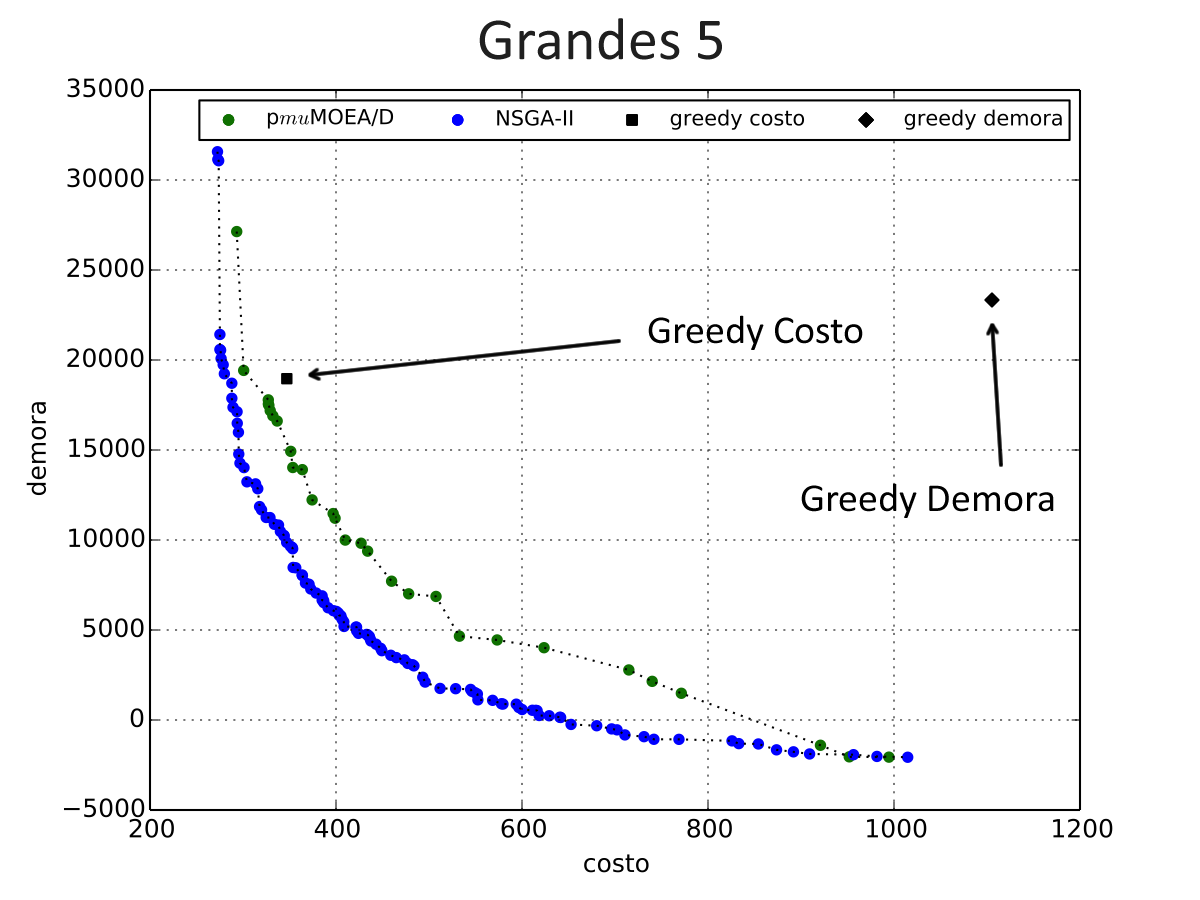
\includegraphics[width=4.5cm,height=3.5cm]{./evaluacion_experimental/fp_comparacion/Gr_5_2.png}\\
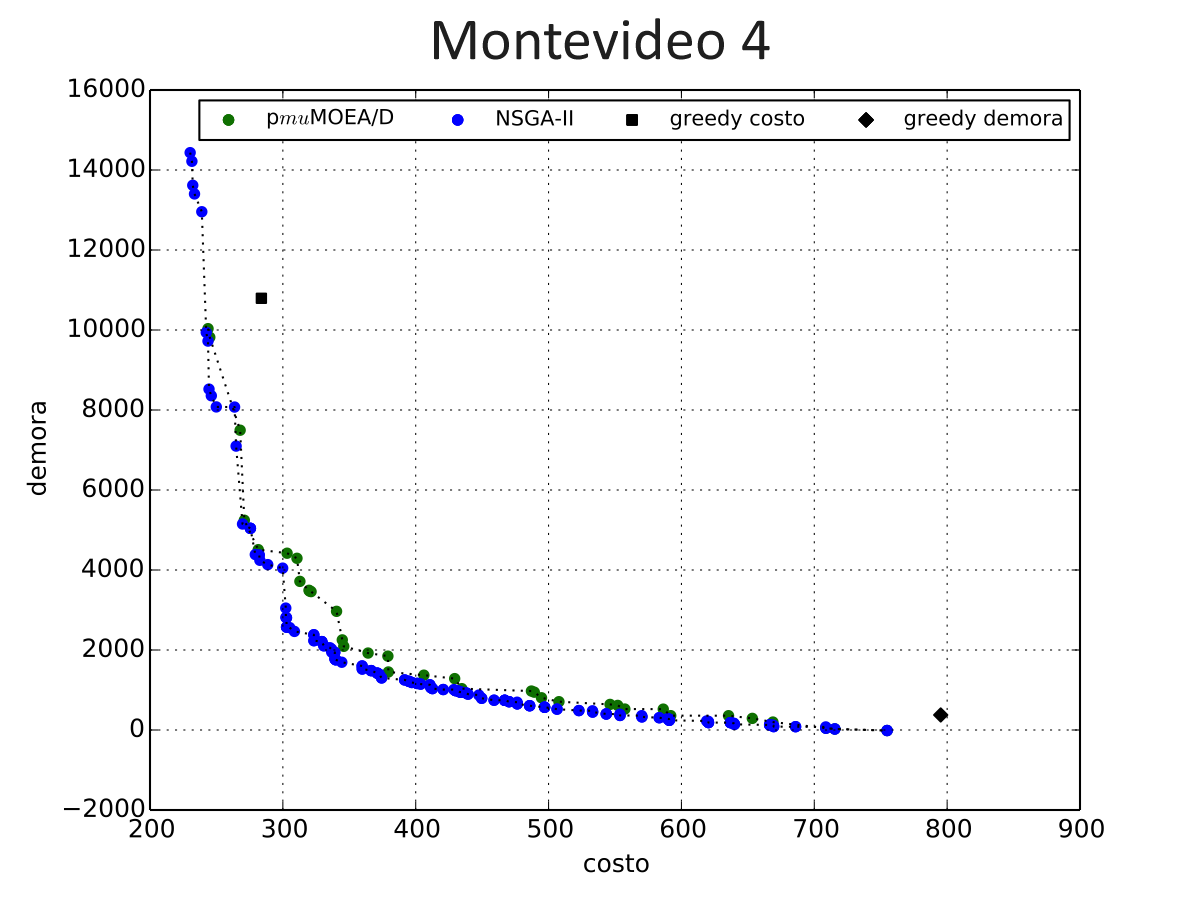
\includegraphics[width=4.5cm,height=3.5cm]{./evaluacion_experimental/fp_comparacion/Mo_4_3.png}
\end{columns}
	
}


% Slide - Planificador de viajes compartidos en línea ==============================================================
\section{Planificador de viajes compartidos en línea} 
\frame{\tableofcontents[currentsection]}

\frame{
	\frametitle{Planificador de viajes compartidos en línea}
	\begin{columns}[totalwidth=\textwidth]
	\column{0.5\textwidth}
	\begin{itemize}
	\item Se ingresa el origen, los destinos y la tarifa (diurna/nocturna).
	\end{itemize}
	\centering
	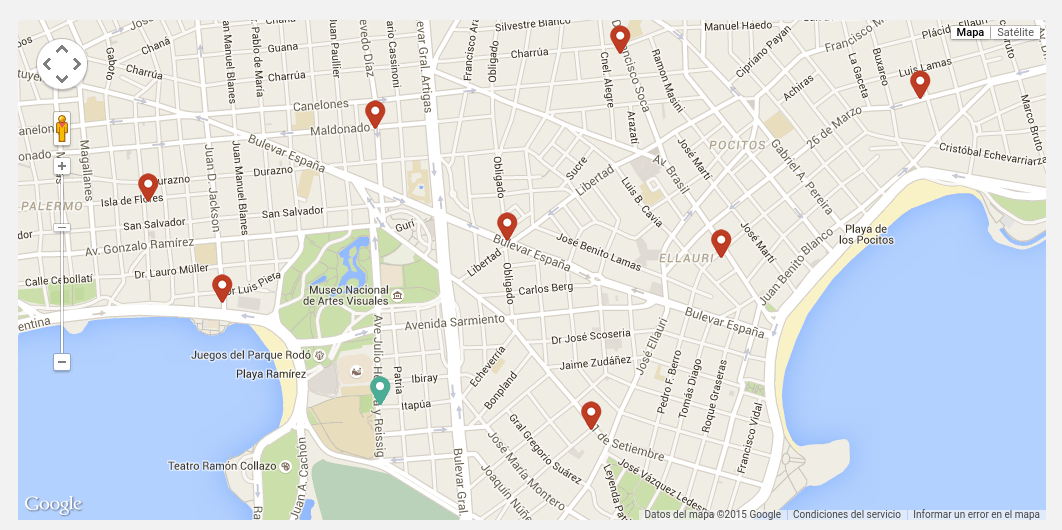
\includegraphics[width=.6\textwidth]{mapa.png}
	\begin{itemize}\pause
	\item Se ejecuta el AE y se muestra la planificación calculada.
	\end{itemize}
	\only<1>{\mbox{\phantom{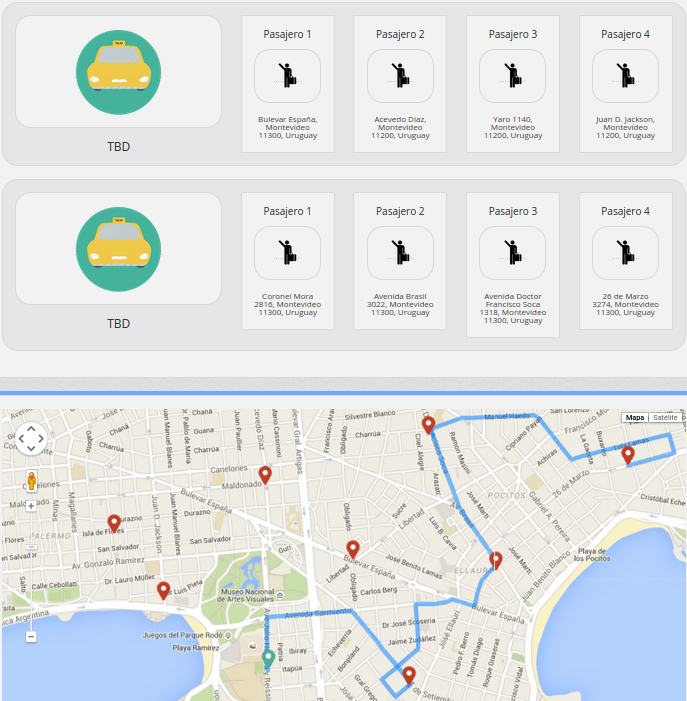
\includegraphics[width=.6\textwidth]{res_total.png}}}}%
	\includegraphics<2->[width=.6\textwidth]{res_total.png}
	\column{0.5\textwidth}\pause
	\centering
	\only<1-2>{\mbox{\phantom{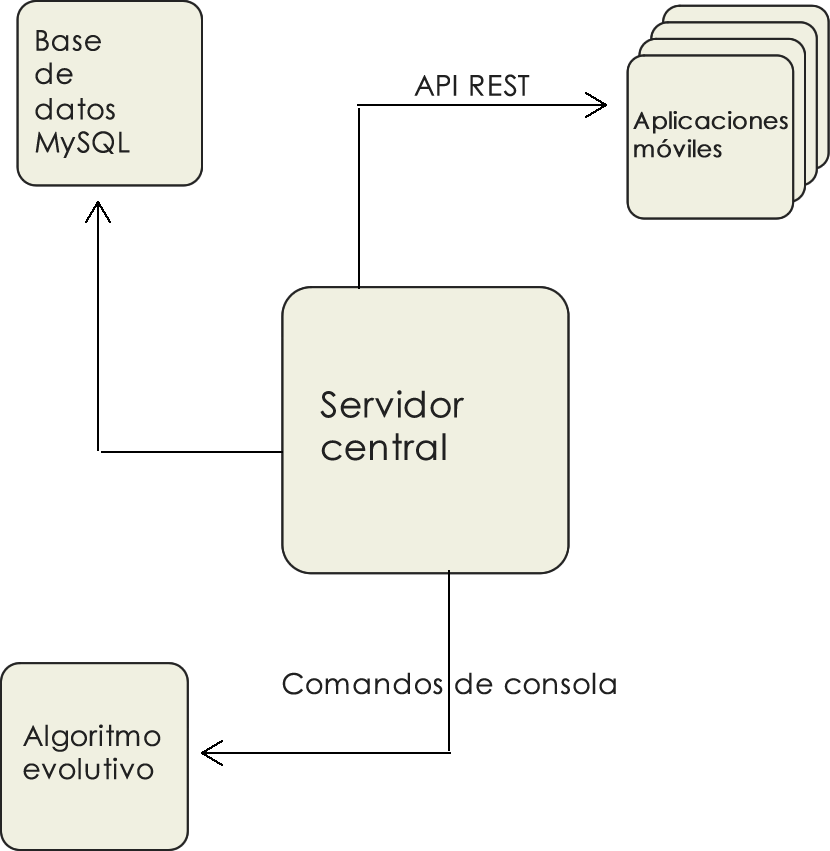
\includegraphics[width=.6\textwidth]{arquitectura.png}}}}%
	\includegraphics<3->[width=.6\textwidth]{arquitectura.png}
	\begin{itemize}
	\item Servidor implementado en Ruby on Rails siguiendo MVC.
	\item Las aplicaciones móviles consumen la API del servidor.
	\item Aplicaciones móviles: desarrollo híbrido vs. desarrollo nativo.
	\end{itemize}
	\end{columns}
}


% Slide - Conclusiones y trabajo futuro ==============================================================
\section{Conclusiones y trabajo futuro} 
\frame{\tableofcontents[currentsection]}

\frame{
	\frametitle{Conclusiones}
	\begin{itemize}
	\item Se relevó la literatura relacionada (CPP, DARP, TPP) y se presentaron dos variantes del problema.\pause
	\item Se implementaron \textbf{cuatro} AE: dos para cada variante del problema.\pause
	\item El análisis experimental se realizó sobre \textbf{instancias realistas}.\pause
	\item Los AE implementados fueron comparados contra algoritmos ávidos.\pause
	\item Variante monoobjetivo: mejoras en costo de hasta \alert{35.9\%} (seqEA) y \alert{41.0\%} (p$\mu$EA) sobre algoritmo ávido.\pause
	\item Variante multiobjetivo: mejoras de hasta \alert{72.8\%} y \alert{101.2\%} (p$\mu$MOEA/D); \alert{75.1\%} y \alert{105.2\%} (NSGA--II) en costo y demora sobre algoritmos ávidos.\pause
	\item Planificador de viajes compartidos en taxis, disponible públicamente en \url{www.mepaseaste.uy}.\pause
	\item \textbf{Cuatro} artículos en conferencias internacionales.\pause
	\item \textbf{Primer premio} del jurado en ``Ingeniería deMuestra 2014'' .
	\end{itemize}
}


\frame{
	\frametitle{Trabajo futuro}
	\begin{itemize}
	\item Implementar NSGA--II con subpoblaciones distribuidas.\pause
	\item Incorporar \textbf{datos realistas del tráfico} para considerar rutas alternativas.\pause
	\item Incorporar datos de la \textbf{disponibilidad de los taxis} en tiempo real.\pause
	\item Mejoras en el planificador de viajes compartidos:\pause
	\begin{itemize}
		\item Mejorar la experiencia de los usuarios.\pause
		\item Desarrollar versiones para dispositivos móviles Android y Windows Phone.\pause
		\item Soportar la variante multiobjetivo.
	\end{itemize}\pause
	\item Estudiar la aplicabilidad de los AE a otros escenarios.\pause
	\item Estudiar otras variantes del problema (e.g., many--to--one, many--to--many).
	\end{itemize}
}

\end{document}\grid